\documentclass[12pt, a4paper]{report}

\usepackage[utf8]{inputenc}
\usepackage[T1]{fontenc}
\usepackage{times}
\usepackage{geometry}
\usepackage{graphicx}
\usepackage{xcolor}
\usepackage{setspace}
\usepackage{titlesec}
\usepackage{fancyhdr}
\usepackage{hyperref}
\usepackage{booktabs}
\usepackage{amsmath}
\usepackage{amsfonts}
\usepackage{amssymb}
\usepackage{array}
\usepackage{multirow}
\usepackage{caption}
\usepackage{tocloft}
\usepackage{pifont}
\usepackage{tabularx}
\usepackage{adjustbox}
\usepackage{float}
\usepackage{cite}


\geometry{
    top=1.0in,
    bottom=1.0in,
    left=1.25in,
    right=1.0in
}

\hypersetup{
    colorlinks=true,
    linkcolor=black,
    citecolor=black,
    urlcolor=blue
}

\onehalfspacing

% Optimized chapter and section spacing for publication quality (~45 pages target)
\titleformat{\chapter}[display]
  {\normalfont\Large\bfseries}{Chapter \thechapter}{8pt}{\LARGE}
\titlespacing*{\chapter}{0pt}{-10pt}{14pt}
\titlespacing*{\section}{0pt}{10pt}{4pt}
\titlespacing*{\subsection}{0pt}{8pt}{3pt}

\captionsetup{font=small, labelfont=bf, skip=6pt}

\pagestyle{fancy}
\setlength{\headheight}{14.5pt}
\fancyhf{}
\fancyhead[L]{\leftmark}
\fancyhead[R]{\thepage}
\renewcommand{\headrulewidth}{0.4pt}

\begin{document}

% =========================================================================
% TITLE PAGE
% =========================================================================
\begin{titlepage}
    \centering
    \vspace*{0.3cm}

    {\LARGE \textbf{
A Closed-Loop Wearable EEG Framework\\[0.3cm]
for Migraine Mitigation\\[0.3cm]
via Binaural Beat Entrainment
}}\\[1.5cm]

    {\large \textbf{By}}\\[0.3cm]
    {\large Abu Hurayra Mahbe -- 0112230043}\\
    {\large Md. Shakibul Hassan Prince -- 0112230048}\\
    {\large Anisa Azmi -- 0112230292}\\
    {\large Jarin Tabassum -- 0112230836}\\
    {\large Mahmudul Mashrafe -- 0112230115}\\[1.5cm]

    {\large Submitted in partial fulfilment of the requirements of the\\ degree of Bachelor of Science in Computer Science and Engineering}\\[1.5cm]

    {\large June 11, 2026}\\[1.2cm]

    \IfFileExists{Images/uiu_logo.png}{%
        
\includegraphics[width=0.22\textwidth]{Images/uiu_logo.png}\\[0.4cm]
    }{%
        \vspace{1.2cm}
    }
    {\large Department of Computer Science and Engineering\\
    United International University}

    \vfill
\end{titlepage}

\pagenumbering{roman}

% =========================================================================
% ABSTRACT
% =========================================================================
\chapter*{Abstract}
\addcontentsline{toc}{chapter}{Abstract}
Migraine is a debilitating chronic neurovascular disorder that affects over one billion people globally. It is characterised by Thalamo Cortical Dysrhythmia(TCD), increased cortical excitability, and sensory habituation anomalies. These can often lead to unwanted side effects, medication overuse headaches, and poor compliance with conventional medication. This Final Year Design Project provides an integrated neuro-engineering approach to migraine treatment using EEG Time  Frequency Classification and neuromodulation using tailored sound. A pipeline was developed to preprocess the data taken from the Carnegie Mellon University(CMU) ultra high density dataset. It contained 128-channel EEG recordings from resting state and sensory stimuli(Auditory SSAEP \& Visual SSVEP). The data was preprocessed using Common Average Referencing (CAR), Bandpass Filtering(1.0--50.0 Hz) and Notch Filtering(60 Hz). The data from the occipital channel (\#80) was transformed into time-frequency spectrograms using a Short-Time Fourier Transform(STFT). The spectrograms were created using a Viridis Colourmap and had a dynamic range of $[-10, +30]$ dB. We then used three different models to classify the data: VGG16, ResNet50 and EfficientNetB7. EfficientNetB7 gave the best results, with an accuracy of 93.75\%, weighted precision of 94.71\%,weighted F1 Score of 93.85\% and MCC of 0.8750. In comparison,VGG16 had an accuracy of 90.63\% and MCC of 0.7985, whilst ResNet50 had an accuracy of 87.50\% and MCC of 0.7410. An algorithm was developed to analyse the RGB Colourmap. Each pixel's RGB value was matched to its nearest colour in the 256-colour Viridis LUT using least Euclidean distance. This allowed an approximate power spectral density ($\mu\text{V}^2/\text{Hz}$) to be extracted from the spectrogram. This provided a way of finding patient specific electrophysiological information such as individual alpha frequency (IAF), alpha deficit (below a 20\%) and Theta to Alpha Ratio (TAR). In a descriptive analysis of resting state participants (12 migraine, 22 control), relative theta power was slightly higher in migraine patients ($15.47 \pm 8.48\%$ vs $13.17 \pm 5.93\%$), whereas relative alpha power and TAR did not show the group level alpha reduction reported in the literature; no statistical tests were performed. Using the individual alpha frequency, a sound generator was used to create customised binaural beats from dual pure tones. These were centred around a carrier frequency of 216 Hz. The beats had a squared half cosine taper of 1.5 seconds to avoid clicking. An example patient (M10) was analysed and had an alpha frequency peak detected at 10.09 Hz. The algorithm also detected an alpha deficit of 7.88\%. A beat was then generated with a precise frequency of 10.09 Hz ($f_{\text{left}} = 210.96$ Hz and $f_{\text{right}} = 221.05$ Hz). The beat was stored as a stereo 16-bit audio file at a sampling frequency of 44.1 kHz. This project creates a technology that allows DNN to be used to detect migraine and create tailored sound to target the auditory cortex. This provides a proof of concept towards a scalable digital solution for migraine; clinical efficacy has not yet been tested.
\newpage

% =========================================================================
% ACKNOWLEDGEMENTS
% =========================================================================
\chapter*{Acknowledgements}
\addcontentsline{toc}{chapter}{Acknowledgements}
We express our deepest gratitude to our project supervisor, \textbf{Dr.~Jannatun Noor Mukta}, for her guidance, academic critique, and continuous encouragement throughout this Final Year Design Project. Her insights into biomedical signal processing and machine learning have shaped the foundation of this work.

We extend our sincere thanks to \textbf{RA Md Abu Obaida Zishan}, our laboratory coordinator, for his technical assistance, practical troubleshooting suggestions, and feedback on algorithmic pipelines. We also express our respect to \textbf{Dr.~Hasan Sarwar}, Head of the Department of Computer Science and Engineering at United International University, and the faculty for providing high-performance computing infrastructure and academic resources.

We are deeply appreciative of the authors of the open-access CMU Ultra-High-Density EEG dataset---Dr.~Alireza Chamanzar, Dr.~Sarah M. Haigh, Dr.~Pulkit Grover, and Dr.~Marlene Behrmann---whose experimental work provided the empirical foundation for our investigations. Finally, we thank our families and teammates for their dedication and support throughout this endeavor.

\newpage

% =========================================================================
% PUBLICATION LIST
% =========================================================================
\chapter*{Publication List}
\addcontentsline{toc}{chapter}{Publication List}

\subsection*{Journal Articles (Prepared / Under Submission)}
\begin{enumerate}
    \item \textbf{A. H. Mahbe, M. S. H. Prince, J. Tabassum, A. Azmi, M. Mashrafe, and J. N. Mukta}, ``Spectrogram-Driven Deep Transfer Learning and Analytical Colormap Inversion for Personalized Binaural Beat Neuromodulation in Interictal Migraine,'' target venue: \textit{IEEE Transactions on Neural Systems and Rehabilitation Engineering} / \textit{Biomedical Signal Processing and Control}, 2026.
\end{enumerate}

\subsection*{Conference Papers (Prepared / Under Submission)}
\begin{enumerate}
    \item \textbf{M. Mashrafe, A. H. Mahbe, M. S. H. Prince, J. Tabassum, A. Azmi, and J. N. Mukta}, ``A Closed-Loop Framework for Interictal Migraine Classification via Convolutional Neural Networks and Individual Alpha Frequency Acoustic Entrainment,'' target venue: \textit{IEEE International Conference on Biomedical and Health Informatics (BHI)}, 2026.
\end{enumerate}


\subsection*{Open-Source Deliverables and Data Artifacts}
\begin{enumerate}
    \item \textbf{FYDP-III Research Artifacts}: Complete Jupyter Notebook repository comprising raw EEG preprocessing (\nolinkurl{1_EEG_CMU.ipynb}), deep transfer learning benchmarks (\nolinkurl{2_Migraine_VGG16_Spectrogram.ipynb}, \nolinkurl{3_Migraine_EfficientNetB7_Spectrogram.ipynb}, \nolinkurl{4_Migraine_ResNet50_Spectrogram.ipynb}), and the spectrogram inversion audio synthesis engine (\nolinkurl{5_spectrogram_binaural_treatment.ipynb}).
    \item \textbf{Audio Prescription Repository}: Cohort-wide synthesized 16-bit 44.1\,kHz stereo WAV binaural beat prescriptions tailored to individual alpha frequencies across all migraine subjects.
\end{enumerate}

\newpage

% =========================================================================
% TABLE OF CONTENTS & LISTS
% =========================================================================
\tableofcontents
\newpage

\listoffigures
\addcontentsline{toc}{chapter}{List of Figures}
\newpage

\listoftables
\addcontentsline{toc}{chapter}{List of Tables}
\newpage

% =========================================================================
% CHAPTER 1: INTRODUCTION
% =========================================================================
\pagenumbering{arabic}
\chapter{Introduction}
\label{ch:introduction}

\section{Project Overview}
\label{sec:project_overview}
Migraine is a long‑term brain problem that shows up as a very strong throbbing pain, in the head. The pain is usually on one side. Is often joined by nausea and a dislike of light and loud noise \cite{Zhang2023,VanDenHoek2024}. One third of people who have migraine feel a warning sign, called aura before the pain starts \cite{Riederer2023}. A study done by the Global Burden of Diseases (GBD) research program found that migraine is one of the causes of years lived with disability (YLD). Migraine is common worldwide. Touches than 1.1 billion people, especially those who are of working age \cite{Petrusic2025,DanelakisStubberud2025}.

Even though migraine is a load on society most treatments focus on medicines like triptans and NSAIDs and on long‑term medicines such as beta‑blockers, topiramate and CGRP receptor blockers \cite{Quartetti2025,Shamsi2024}. Yet than 40% of people with migraine find these medicines do not work, cause side effects or are not safe for them \cite{Shamsi2024}. In addition taking these medicines often can create medication overuse headaches (MOH) turning a migraine into a severe chronic one \cite{GomezPilar2022}. For this reason we urgently need non‑drug ways to treat migraine, such, as technology.
Quantitative electroencephalography (qEEG) reveals that migraineurs exhibit significant neurophysiological disturbances during interictal (headache-free) periods, prominently \textit{thalamocortical dysrhythmia} (TCD) and pervasive cortical hyperexcitability \cite{VanDenHoek2024,AbdulhusseinAldeen2024}.These abnormalities occur through abnormal spectral power distribution, non-habituation to repetitive visual/auditory stimuli, and pronounced posterior alpha waves (8.0--13.0~Hz) suppression \cite{chamanzar2021uhd,Zhang2023,FrimpongManson2024}. Additionally, the method of acoustic neuromodulation through \textit{binaural beats} has become known as a possible way of non-invasively influencing the cortex through the phenomenon of frequency-following response (FFR) in the brainstem \cite{Oster1973,Wahbeh2007,Ingendoh2023}.

Still, current knowledge in this area is insufficient, as diagnostic research is mostly concerned with offline machine learning classification without any subsequent treatment \cite{aslan2023migrainecnn,orhanbulucu2023hybrid}, while commercially available binaural beat solutions generate a general-purpose audio stimulus of fixed frequencies (for example, a common 10~Hz) regardless of patient's individual alpha frequency (IAF) and power loss \cite{CoronaGonzalez2021,KahathuduwaBlume2025}. This Final Year Design Project seeks to solve this problem through the creation of a complete software solution combining deep learning-based detection of interictal migraines from 2D STFT spectrogram images with a colormap inversion algorithm, which allows for the extraction of IAF value and thus allows for the synthesis of a personalized audio prescription.

\section{Motivation}
\label{sec:motivation_objectives}
This research addresses both necessities and computational engineering opportunities:

\begin{itemize}

    \item \textbf{Non-Pharmacological Therapy}: Explore a side-effect- alternative, to medication that seeks to restore balance, in brain wave patterns \cite{Quartetti2025,Shamsi2024}.

    \item \textbf{Objective Biomarker Diagnostics}: Replace memory of symptoms with qEEG signals that show brain hyperactivity and thalamocortical slowing \cite{chamanzar2021uhd,Petrusic2025}.

    \item \textbf{Time-Frequency Computer Vision}: Use 2D time-frequency spectrograms feeding them into trained deep convolutional networks (CNNs) to extract strong features reliably \cite{orhanbulucu2023hybrid,Rakhmatulin2024}.

    \item \textbf{Patient-Specific Resonant Entrainment}: Adjust binaural beat frequencies to match each patient’s alpha frequency (IAF) so that cortical phase-locking is maximized \cite{Melnichuk2025,Hamid2025}.

\end{itemize}

\section{Objectives}
The specific project objectives are:
\begin{enumerate}
    \item Build a preprocessing pipeline for 128‑channel ultra‑high‑density EEG (CAR, 1.0–50.0~Hz FIR bandpass, 60~Hz notch filtering).
    \item Generate 2D STFT spectrogram images, from / channel recordings during resting‑state, SSAEP and SSVEP paradigms.
    \item. Benchmark deep transfer learning models (VGG16, ResNet50 EfficientNetB7) for automated migraine detection.
    \item Formulate a RGB colormap inversion algorithm that converts pixel intensities into linear power spectral density ($\mu\text{V}^2/\text{Hz}$).
    \item Extract patient‑specific IAF, Alpha Deficits and Theta‑to‑Alpha Ratios (TAR), from the data.
    \item Engineer an synthesis engine that generates click‑free dichotic stereo binaural beat prescriptions modulated to each patient’s IAF.
    \item Evaluate the framework through population cohort analytics and single‑subject case studies.
\end{enumerate}

\section{Methodology}
\label{sec:methodology_ch1}
The methodology developed in this project constitutes a multi-stage, closed-loop computational and neuro-acoustic engineering pipeline designed to bridge automated interictal migraine diagnosis with personalized therapeutic intervention:
\begin{enumerate}
    \item \textbf{Data Preprocessing and Artifact Suppression}: High-density 128-channel EEG recordings ($f_s = 2048$~Hz, downsampled to 512~Hz) are referenced against Common Average Reference (CAR), filtered through a zero-phase 4th-order Butterworth bandpass filter (1.0--50.0~Hz) to isolate physiologically salient oscillations, and processed with a 60~Hz notch filter to eradicate power-line interference.
    \item \textbf{Time-Frequency Transformation and Channel Selection}: Signal epochs are extracted from occipital channel \#80 (Oz/O1 boundary under the IFCN standard, exhibiting the highest signal-to-noise ratio for visual and alpha rhythm dynamics). Short-Time Fourier Transform (STFT) with a 256-point Hamming window and 50\% overlap transforms the 1D temporal voltages into high-resolution 2D time-frequency spectrogram images rendered under the Viridis colormap standard ($224 \times 224$ pixels).
    \item \textbf{Deep Transfer Learning Classification}: Spectrogram images are fed into pre-trained deep convolutional neural networks (VGG16, ResNet50, and EfficientNetB7) fine-tuned for binary classification between interictal migraine patients and healthy controls, circumventing manual feature engineering.
    \item \textbf{Color-to-Power Inversion Algorithm}: An analytical inverse mapping algorithm evaluates the Euclidean distance of RGB pixel coordinates against the normalized 256-level Viridis lookup table, accurately decoding quantized pixel intensities back into continuous, calibrated linear Power Spectral Density ($\mu\text{V}^2/\text{Hz}$) across the 1.0--50.0~Hz spectrum.
    \item \textbf{Neuro-Biomarker Extraction}: The reconstructed PSD curve is algorithmically interrogated to determine the patient's exact Individual Alpha Frequency (IAF, peak power in the 8.0--13.0~Hz band), Alpha Deficit relative to normative control baselines, and Theta-to-Alpha Ratio (TAR).
    \item \textbf{Personalized Acoustic Entrainment}: A dichotic stereo synthesis engine constructs dual pure sine waves ($f_{\text{left}} = f_c - \Delta f / 2$, $f_{\text{right}} = f_c + \Delta f / 2$) centered at an ergonomic carrier frequency ($f_c = 216.0$~Hz, near A3 concert pitch) with the interaural frequency differential $\Delta f$ matched precisely to the detected IAF. A squared half-cosine taper envelope ($T_{\text{fade}} = 1.5$~s) eliminates auditory switching clicks, exporting high-fidelity 16-bit uncompressed stereo audio for clinical and home therapeutic administration.
\end{enumerate}

\section{Project Outcome}
\label{sec:project_outcome}
The successful execution of this project yields several tangible scientific, technological, and translational outcomes:
\begin{itemize}
    \item \textbf{High-Accuracy Single-Channel Diagnostic Framework}: Demonstrated a deep transfer learning model (EfficientNetB7) capable of discriminating interictal migraineurs from healthy subjects with 93.75\% accuracy, 100\% precision, 0.933 F1-score, and a Matthews Correlation Coefficient of 0.875 using only occipital channel \#80, validating the feasibility of minimal-montage wearable screening.
    \item \textbf{Novel Spectrogram Inversion Formulation}: Developed and validated an analytical RGB-to-PSD decoding engine that reconstructs continuous linear power spectral densities from 2D visual spectrograms with near-perfect correlation ($r > 0.998$) against Welch numerical transforms, bypassing raw signal transmission constraints in distributed digital health systems.
    \item \textbf{Tailored Closed-Loop Digital Therapeutic}: Formulated an automated pipeline translating empirical EEG biomarkers into customized binaural beat audio prescriptions, providing patients with individual-specific alpha entrainment capable of restoring thalamocortical desynchrony.
    \item \textbf{Foundation for Low-Cost Wearable Neurotechnology}: Established the algorithmic and architecture specifications required to transition from expensive (\$25,000+) clinical 128-channel caps to an affordable ($<\$250$), consumer-grade single-electrode dry headband.
    \item \textbf{Reproducible Open-Source Computational Artifacts}: Provided a modular, fully documented codebase complying with IFCN electrode standards and BIDS neuroimaging specifications, facilitating clinical trial replication and cross-institutional research.
\end{itemize}

\section{Organization of the Report}
\label{sec:organization}
The rest of this report is organized as follows: Chapter~\ref{ch:background} covers basics a five-domain literature review and a thorough analysis of research gaps. Chapter~\ref{ch:project_design} explains the process, from start, to finish including dataset setup, signal processing, deep transfer learning models, colormap inversion and binaural audio synthesis. Chapter~\ref{ch:experimental_results} shows the results, including classification performance, confusion matrices, ROC curves, a detailed case study of M10 and group-level analysis. Chapter~\ref{ch:design_constraints} looks at engineering standards, safety and design limitations. Chapter~\ref{ch:conclusion} wraps up with findings, limitations and ideas for work.

% =========================================================================
% CHAPTER 2: BACKGROUND & LITERATURE REVIEW
% =========================================================================
\chapter{Background and Literature Review}
\label{ch:background}

\section{Preliminaries}
\subsection{Neurophysiological Foundations of Migraine}
\label{sec:neuro_foundations}
 Migraine involves complex neurovascular dysfunction, including repetitive trigeminovascular excitation, cortical spreading depression (CSD) and disrupted sensory processing \cite{Zhang2023,VanDenHoek2024}. The hallmark feature of the migraine brain during the interictal phase is thalamocortical dysrhythmia (TCD) \cite{VanDenHoek2024,AbdulhusseinAldeen2024}. Under normal physiological conditions, the thalamus acts as a sensory gateway to filter afferent signals. Synchronous alpha oscillations (8.0 13.0 Hz) generated by feedback loops within the thalamic reticular nucleus drive the cortex \cite{Zhang2023}. However, it is thought that deinactivation of low threshold T type calcium channels can cause irregular low frequency bursting of the thalamic neurons at theta range (4.0 8.0 Hz). This causes irregular thalamocortical driving, reduced posterior alpha power and unmasking of hyperexcitable cortex. 


One hallmark electro-physiological feature of TCD is the \textit{ inability to habituate} to repeated sensory stimulation \cite{chamanzar2021uhd,AbdulhusseinAldeen2024} . In healthy individuals, reduced amplitude in evoked potentials can be seen when exposed to continuous visual and auditory stimuli. However, migraine suffers show poor habituation or sensory sensitisation.


\subsection{Principles of Binaural Beat Neuromodulation}
\label{sec:binaural_principles}
Binaural beats is a third, rhythmic, pulsing tone when two pure tones of nearby frequencies are presented concurrently, one to each ear through stereo headphones ($f_1$ and $f_2$)  \cite{Oster1973}. These signals sum in the brainstem region of the superior olivary complex (the superior olivary nuclei) called the "medial superior olive" (MSO) which functions in sound location by the detection of interaural phase difference (IPD) \cite{Wahbeh2007}:
\begin{equation}
    f_{\text{beat}} = |f_1 - f_2|
    \label{eq:binaural_beat_freq}
\end{equation}
This phase-locked activity propagates through the lateral lemniscus and inferior colliculus to the medial geniculate of the thalamus and auditory cortex to give a \textit{frequency-following response} (FFR) \cite{Ingendoh2023,Shamsi2024}. When in the alpha range ($f_\text{beat}\in [8.0,13.0]$~Hz), binaural beats are theorized to elicit resonant thalamocortical entrainment, re-establishing sensory gating and reducing cortical hyperexcitability \cite{CoronaGonzalez2021,Melnichuk2025,battu2025longterm}; direct clinical evidence in migraine is lacking.

\section{Structured Literature Review}
\label{sec:literature_review}
To give a full background to the work carried out during this thesis, we carried out a literature review in each of these 5 areas; (1) EEG and Biomarkers for Migraine, (2) Binaural Beats and Brainwave Entrainment, (3) Wearable EEG Platforms and Digital Phenotyping, (4) Feature Extraction and Machine Learning Approaches, and (5) Binaural Beat Generation and Acoustic Neuromodulation Systems.

\subsection{EEG and Biomarkers for Migraine}
\label{subsec:lit_eeg_biomarkers}
For some decades, researchers have examined the potential of using EEG as a migraine biomarker. These initial studies showed migraine patients have more delta/theta activity during their attacks and more beta activity during remissions. Recent studies have utilised quantitative EEG (qEEG) approaches and confirmed that patients with migraine do have evidence of cortical hyperexcitability. This includes reduced alpha activity, high frequency oscillations and interhemispheric coherence issues  \cite{VanDenHoek2024}. MEG studies have localised these cortical regions to the occipital, parietal and prefrontal regions of the cortex which are associated with sensory perception and pain processing. Furthermore, it was shown that quantitative EEG changes could be detected up to 36hrs before migraine onset, meaning it could be used as a prodromal migraine biomarker  \cite{Kim2023}. The study performed by Joshi et al., utilised EEG to create spiking and convolutional spiking neural networks (CSNN) to detect stress. Their aim was to create temporal models for accurate predictions whilst also being efficient with energy. They obtained an accuracy of 98.61\%, sensitivity of 100\% and F1-score of 98.60\% using their CSNN. This resulted in a fast processing time and compact model for wearable devices \cite{JoshiMatharu2025}. Van Den Hoek et al., provided an overview of spontaneous activity, evoked potentials and treatment induced changes in brain activity across the migraine cycle to determine if EEG can be used as a vulnerability biomarker \cite{VanDenHoek2024}. They highlighted that there were consistent changes detected within the preictal period including increased theta/alpha power, slowed activity and connectivity. However, no one secure biomarker was identified. Future work will involve using wearable EEG devices in homes and conventional methods to investigate biomarker vulnerability. Zhang et al., investigated various aspects of EEG including resting state, evoked potentials, connectivity, microstates and machine learning classifiers to understand its potential to be used in migraine \cite{Zhang2023}. Previous changes were observed including increased alpha slowing, increased delta/theta activity, changed networks and helpful ML classifiers. However, issues included individual variability and small sample sizes. Frimpong-Manson et al., analysed EEG data and used prospective and retrospective analysis to find objective migraine signatures. They observed reproducible headache biomarkers including increased occipital 12-13Hz activity during the interictal period \cite{FrimpongManson2024}. They showed their KNN and SVM ML classifiers were able to accurately classify migraine patients and controls (87.2\%). This supports using occipital alpha as a potential headache biomarker. Quartetti et al., completed a systematic review of 36 studies to identify lifestyle factors incident to episodic migraines. They concluded that ketogenic diets, supplements and physical activity are evidence-based ways to reduce the number of migraine attacks. However, no EEG headache biomarkers or ML models have been directly tested \cite{Quartetti2025}. Zebhauser et al., completed a meta-analysis of 27 studies using EEG/MEG technology on migraine patients. They identified a potential EEG migraine signature including increased theta activity and decreased alpha-beta connectivity between brain regions to detect pre-symptomatic migraine. However, there were large methodological issues including comorbidities, small samples and different methods  \cite{Zebhauser2024}. Studies looking at Steady-State Visual Evoked Potentials (SSVEPs) have shown rhythmic stimulation can act as a pacemaker for thalamocortical dysrhythmia in migraine  \cite{AbdulhusseinAldeen2024}. Gomez-Pilar et al., completed a systematic review and found evidence from EEG, MRI and PET imaging showing different activity within the brain networks of chronic and episodic migraine patients  \cite{GomezPilar2022}. Consistent differences were found within the fast EEG/MEG bands and pain/ emotion-related networks. This suggests that multimodal functional biomarkers may be used as objective biomarkers to determine if someone is at higher risk of developing chronic migraine. Riederer et al., completed a narrative review of EEG/MRI characteristics of migraine aura to help neurologists perform differential diagnosis. Simple visual aura usually shows normal scalp EEG. However, complex aura usually shows focal slowing/suppression during the acute phase  \cite{Riederer2023}. Göker proposed a novel automated migraine detection system using Welch’s method (1.0-49.0Hz). They showed their BiLSTM (128-channels) had an overall accuracy of 95.99\%, sensitivity of 0.96, specificity of 0.95 and F1 score of 0.96. This outperformed other classifiers such as RF, SVM and LDA using the same EEG data  \cite{Goker2023}. Kedgan et al., completed a systematic review and meta-analysis of the prevalence of EEG patterns during the aura, headache, post-headache and interictal phases of hemiplegic migraine. They found low amplitude contralateral background activity during the aura phase. During the headache phase focal slowing was observed. During interictal periods mostly normal EEG was observed with evidence of genotype differences  \cite{Kedgan2025}. Raghuraman and Joshi performed a scoping review on using EEG for diagnosing and classifying migraine. They found evidence of cortical hyperexcitability, poor habituation, abnormal microstates (reduced class C, increased class B/D) and automatic AR-Burg models (up to 88.7\% accuracy). However, they concluded there were issues with methodology and that current research is focusing on migraine without aura so an automated etiology-based diagnostic system cannot be reliably established  \cite{RaghuramanJoshi2024}. Kim et al., completed an evaluation of qEEG as a potential migraine biomarker. They used z-score maps on 720 subjects and found migraine patients had increased overall absolute power. Patients had high absolute power in the beta frequency band (25-30Hz) which correlated with clinical improvement  \cite{Kim2023}.


\subsection{Binaural Beats and Brainwave Entrainment}
\label{subsec:lit_binaural_beats}
A steady state Continuous Performance Task (CPT) was implemented to investigate the effects of varying beta (16~Hz)  and gamma (40~Hz)  binaural beats on sustained attention  \cite{Melnichuk2025} . Consistent entrainment was observed across all EEG measures with gamma binaural beats providing the most consistent results. An increase in hit rate was also observed when optimum acoustic stimuli was utilised (40 Hz beat, 340 Hz carrier, 340 Hz white noise mask, beat delivery at task start). A randomised cross-over trial was carried out with 6, 10 and 25 Hz binaural beats to investigate effects on college students  \cite{Yang2025} . A decrease in heart rate and blood pressure was observed across all binaural beat conditions. The 25 Hz binaural beat provided the greatest parasympathomimetic effect with both a decrease in normalised low frequency power, and an increase in normalised high frequency power. However, no EEG data was recorded. A meta-analysis of 15 randomised control trials investigating binaural beats for the peri-operative period found significant reductions in anxiety ([SMD] $-1.0$ to $-1.4$). Moderate improvements in pain and haemodynamics were also reported \cite{Xiong2025}. A customised EEG guided real-time binaural beat was created and found to improve relaxation and cognitive performance when compared to controls  \cite{KahathuduwaBlume2025}. A systematic review showed that alpha and delta-alpha binaural beats can be effective for reducing acute procedural pain. Results are inconsistent for chronic pain \cite{Shamsi2024}. Stationary binaural beats, panning sounds and pure tone beeps were investigated using wearable EEG. Panning sounds provided greater relaxation and modulation of the cortex  \cite{Sudre2024}. 14 EEG studies were reviewed and only 5 of them provided statistically significant entrainment. None of them were convincing for the beta range \cite{Ingendoh2023}. A study looking at 0.25 Hz and 1.0 Hz beats during daytime naps found that 0.25 Hz stimulation reduced the time taken to enter slow wave sleep (N2/N3) without causing excessive phase locking \cite{Fan2024}. Binaural beats were used during cadaveric dissection. It was found that auditory stimuli helped students manage acute emotional stress with significant reductions in perceived anxiety when compared to controls \cite{Mosheshe2024}. Long and short binaural beat exposure times were investigated. Long exposure times significantly reduced heart rate and LF/HF ratios whilst improving mood scores using the Brunel Mood Scale (BRUMS) \cite{ChockboondeeJatupornpoonsub2023}. Delta binaural beats were shown to improve quality of sleep and post-sleep mood amongst pilots \cite{Dabiri2022}. Functional near-infrared spectroscopy (fNIRS) was used with 16 Hz binaural beats during Stroop tasks. A 44\% reduction in salivary alpha amylase was seen with increased prefrontal activation and faster responses \cite{AlShargie2022}. Gamma and alpha power increased whilst delta was reduced when using 40 Hz binaural beats \cite{WangZhang2022}. A meta analysis looking at binaural beats and cognitive function showed small improvements in memory and attention \cite{BasuBanerjee2023}. Alpha binaural beats were shown to cause activation in the parietal occipital regions of the brain with increased cognitive processing when compared to white noise \cite{Hamid2025}.
 

\subsection{Wearable EEG Platforms and Digital Phenotyping}
\label{subsec:lit_wearable_systems}
Petr\v{s}i\'{c}~\cite{Petrusic2025} mapped out the unpolished state of the art in EEG-based brain--computer interface (BCI) technology as a scalable emerging neural monitoring and assistive rehabilitation paradigm that offers in the wild neural signal acquisition without the clinical risks of invasive systems. The author further classified wearable EEG topologies to be scalp-EEG, forehead-EEG, and ear-EEG. While scalp-EEG systems attain 90--96\% motor imagery and cognitive classification accuracy, Petru\v{s}i\'{c} pointed out important limitations including motion artifact sensitivity, inter-subject variability, unstable electrode impedance, and benchmarking inadequacy.He et al.~\cite{He2023} performed a comprehensive market analysis of commercial wireless EEG systems, which revealed a high heterogeneity in hardware specification (channel count, sampling rate, battery life, and cost from \textdollar 240 to \textdollar 30,000), although the heterogeneity characterizes rapid evolution. The authors emphasized the significance of the lack of standards in hardware validation, artifact management, and algorithm benchmarking for in the wild use. In sequence, Muhammad et al.~\cite{Muhammad2023} proposed a low cost OpenBCI-based 16-channel headset that achieved 82.9\% classification accuracy with a setup time of $2.0\pm 0.5$ minutes and cost an estimated \textdollar 299.Interestingly, their reduced configuration of only 3 channels achieved similar 82.0\% accuracy with 69.1\% channel selection frequency, highlighting the potential of sparse montages to retain information if spatially accurate over the sense of cortical information. Danelakis et al.~\cite{DanelakisStubberud2025} built on the wearable narrative by evaluating digital phenotyping, the digital integration of wearable sensors, smart-phone tracking, and machine learning for head trauma and headache disorder detection at home, which gave classification accuracy from 62\% to 99.7\%, although pitfalls were still evident from small cohorts, overfitting, noise, and external validation limit. Large focus was on reduced feature space for near-real-time prediction ($82\%$ accuracy), and analysis of physical activity across migraine states ($p < 0.01$ to $p < 0.001$).Together, these studies reaffirm the importance of single/sparse-channel machine learning models \cite{Petrusic2025,He2023,DanelakisStubberud2025}.

\subsection{Feature Extraction and Machine Learning Approaches}
\label{subsec:lit_feature_extraction}
Yuvaraj et al.~\cite{Yuvaraj2023} studied the recognition of mental and emotional states using statistical, wavelet, fractal dimension, Hjorth, and higher-order statistics (HOS) features from EEG and showed that using Fractal Dimension features with a CART classifier can reach around 85\% accuracy (near-term feasibility). Kalashami et al.~\cite{Kalashami2022} extracted 344 handcrafted EEG features (including spectral band powers, hemispheric asymmetry, time-domain measures) and augmented the feature space with 5{,}000 synthetic samples generated with Conditional Wasserstein Generative Adversarial Networks (CWGAN), allowing deep neural networks to classify EEG signals with 67.4\% and 71.9\% accuracy for valence and arousal, respectively. Luo et al.~\cite{Luo2024} used 8-level wavelet packets (Daubechies \texttt{db4}) reconstructed from EEG during virtual reality motion sickness to classify with a Gated Recurrent Units (GRU) network and achieved 84.9\% accuracy and high correlation coefficients (Pearson $\text{PLCC} \approx 0.90$, Spearman $\text{SROCC} \approx 0.92$).Rakhmatulin et al.~\cite{Rakhmatulin2024} show the utility of compact CNN architectures such as EEGNet, and cascaded TS-SEFFNet, for feature extraction from preprocessed EEG signals, at accuracies over 90\% for motor imagery and P300 paradigms while keeping parameter counts low. Chaddad et al.~\cite{Chaddad2023} give a detailed review of signal processing pipelines (from adaptive filters to time-frequency analysis, HOS, and non-linear complexity measures) for EEG, reporting 90--99\% accuracy for SVMs and CNNs using curated time-frequency features across neurological applications. Singh and Krishnan~\cite{Singh2023} identified broad trends in feature extraction: spatial filters such as Common Spatial Pattern (CSP) variants yield 80--95\% accuracy for BCI paradigms using multi-channel EEG, while time-frequency transforms (STFT and wavelet transforms) excel for localized sensory evoked potentials and oscillation slowing.

\subsection{Binaural Beat Generation and Acoustic Neuromodulation Systems}
\label{subsec:lit_binaural_generation}
To close the gap between EEG diagnostic classification and acoustic therapy, recent neuro-engineering research revealed the implementation details of 1) binaural beat creation, 2) carrier frequency selection, 3) individual alpha frequency (IAF) optimization, and 4) clinical efficacy for a variety of migraine markers. Orhanbulucu et al.~\cite{orhanbulucu2023hybrid} used time-frequency representations (short-time Fourier transform spectrograms and continuous wavelet transform scalograms) coupled with pre-trained deep CNNs (Alex Net and ResNet50) on the 128-channel CMU ultra-high-density EEG data set in the interictal migraine classification vs. healthy control experiment, and analyzed the effects of sensory stimuli (visual steady-state visual evoked potentials and auditory steady-state evoked potentials) from the 2D imagery: they got the best diagnostic accuracy of 94.70\% using 2D images, which implied that 2D visual spectrograms encode localized cortical hyperexcitability and thalamocortical dysrhythmia. Aslan~\cite{aslan2023migrainecnn} applied a common continuous wavelet transform time-frequency scalogram with a custom deep 2D CNN on the same CMU 128-channel data set, combined with an analysis of spectral energy mapping across the entire scalp, proved that deep CNNs can classify up to 100\% accuracy using individual-scalogram segments, which demonstrated the strong class separability of wavelet spectral biomarkers for interictal migraine detection. Regarding clinical efficacy, Li et al.~\cite{li2023modulating} evaluated the electrophysiological effect of personalized alpha peak frequency (iAPF, also called IAF) in acoustic stimulation, showing that when the beat frequency $f_\text{beat} = \left|f_1 -f_2\right|$ was tuned exactly to the subject's intrinsic resting alpha peak, the phase-locking value (PLV) was significantly higher and the spectral thalamocortical entrainment was significantly stronger, than with a typical fixed-frequency beat (e.g. Strictly 10.0~Hz); their empirical experiments revealed that the beat frequency must be personalized to reach the optimal spectral entrainment. Building on this, Batt\`u et al.~\cite{battu2025longterm} demonstrated a pilot study on long-term binaural beat therapy with 2Hz personalized alpha stimulation: multivariate EEG results showed that the brain activity can be modulated by the binaural beat, and that there was a sustained effect for days after stimulation, with the strongest influence at frontal electrode locations, while binaural beat perception was reported to decline quickly when the carrier frequency was raised over 1000Hz, which supported the low-carrier property of the beneficial therapy. On the diagnostic side, Hsiao et al.~\cite{hsiao2024brainstem} measured somatosensory evoked EEG responses on 342 participants (113 normals, 106 chronic and 123 episodic migraineurs), showed that the brainstem and cortical amplitude were both reduced with increased brainstem--cortex effective connectivity in migraineurs, and achieved the migraine vs. control accuracy of approximately 76\% to 87\% on test SVM classifiers, providing evidence that sensory-induced EEG may be a symptom-based classifier for migraine, even without any migraine therapy.

\subsubsection{Comparative Synthesis of Binaural Beat Generation Studies}
Table~\ref{tab:lit_comparison} summarizes what these five benchmark papers achieved, in addition to the proposed framework. Two high-performance deep learning systems with 2D time-frequency representations (STFT and CWT)~\cite{orhanbulucu2023hybrid, aslan2023migrainecnn} established STFT-based and CWT-based systems for 2D time-frequency representations, respectively. Both systems are designed solely as offline diagnostic tools without any therapeutic feedback, as opposed to the other two papers that provided the physiological feasibility of the personalized alpha-range binaural stimulation using open-loop acoustic protocols that compute the stimulation frequencies using a manual calculation of features based on the image (the ICA decomposition of the EEG data in~\cite{li2023modulating} and sensory-evoked EEG in~\cite{battu2025longterm}).The last one~\cite{hsiao2024brainstem} found EEG responses to sensory stimuli coupled with machine learning for the detection of migraine, but not in a feedback loop.

\begin{table}[htbp]
\centering
\caption{Comparative Synthesis of Literature and Proposed Closed-Loop Framework}
\label{tab:lit_comparison}
\begin{adjustbox}{width=0.98\textwidth}
\begin{tabular}{lcccccc}
\toprule
\textbf{Study} & \textbf{Modality / Channels} & \textbf{Signal Representation} & \textbf{Core Methodology} & \textbf{Reported Metric} & \textbf{Therapeutic Loop} & \textbf{Personalized IAF} \\
\midrule
Chamanzar et al. (2021) \cite{chamanzar2021uhd} & UHD-EEG (128-ch) & Phase Locking / Coherence & Statistical Hypothesis & Coherence Biomarkers & None & None \\
Orhanbulucu et al. (2023) \cite{orhanbulucu2023hybrid} & UHD-EEG (128-ch) & STFT / CWT Images & AlexNet / ResNet50 & 94.70\% Acc & None & None \\
Aslan (2023) \cite{aslan2023migrainecnn} & UHD-EEG (128-ch) & CWT Scalograms & Custom Deep CNN & 100.0\% Acc & None & None \\
Auditory EEG (32-ch) & Spectral Phase-Locking & Personalized Tone Synthesis & $p < 0.01$ PLV Gain & Open-Loop & IAF Peak Matched \\
Batt\`u et al. (2025) \cite{battu2025longterm} & Scalp EEG (pilot) & Multivariate EEG Features & Long-Term Personalised Alpha BB & Sustained Post-Stimulation Effects & Open-Loop & Personalised Alpha \\
Hsiao et al. (2024) \cite{hsiao2024brainstem} & Somatosensory Evoked EEG (342 subj.) & Evoked Amplitude / Connectivity & SVM Classification & 76.2--87.0\% Acc (Indep. Test) & None & None \\
\textbf{Proposed Framework} & \textbf{UHD-EEG / Ch \#80} & \textbf{STFT Viridis Spectrogram} & \textbf{EfficientNetB7 + LUT Inversion} & \textbf{93.75\% Acc (0.875 MCC)} & \textbf{Closed-Loop Audio} & \textbf{Exact IAF Tuning} \\
\bottomrule
\end{tabular}
\end{adjustbox}
\end{table}

\section{Research Gap Analysis}
\label{sec:gap_analysis}
Although marked advances have been reported in the available literature, there remain critical gaps in the technology and methods that limit clinical translation and enable the realization of intelligent closed-loop therapeutics.


There are major flaws in all of the included work limiting translation to the clinic. Joshi et al.~\cite{JoshiMatharu2025} used a Physio Net database that did not contain data from migraine patients in several neurological cohorts, and neuromorphic hardware not cleared for clinical use. Van den Hoek et al.~\cite{VanDenHoek2024} lacked meta analysis, gamma band studies, proof of use in the ambulatory setting, wearable techniques, and relatively standardized data collection.

Zhang et al.~\cite{Zhang2023} and Raghuraman and Joshi~\cite{RaghuramanJoshi2024} both had inconsistent EEG acquisition methods, small samples and visual habituation effects so found very hard to replicate. Frimpong-Manson et al.~\cite{FrimpongManson2024} had small prospective samples in patients still on acute treatment, with inconsistent interval controls and blended migraine subtypes (migraine with and without aura). Quartetti et al.~\cite{Quartetti2025} had inconsistent study designs, no consideration of confounding lifestyle factors, and no direct EEG machine learning linkage. Zebhauser et al.~\cite{Zebhauser2024} lacked blinded trials, had significantly disparate study methodologies, and a small average (62) sample.

Abdulhussein et al.~\cite{AbdulhusseinAldeen2024} were limited by scalp volume conduction hindering potential to distinguish deep thalamic pacing from superficial cortical reverberation; Gomez-Pilar et al.~\cite{GomezPilar2022} lacked longitudinal cross-validation to follow migraine chronification; Riederer et al.~\cite{Riederer2023} merely investigated atypical aura while other studies emphasized episodic migraineurs; Göker~\cite{Goker2023} considered high-dimensional 128-channel BiLSTM models with holdout splits at risk of overfitting; Kedgan et al.~\cite{Kedgan2025} used primarily case series limited to hemiplegic migraine; Kim et al.~\cite{Kim2023} used single-center qEEG data without adequately controlling medication wash-out periods.

For brainwave entrainment and binaural beats \cite{Melnichuk2025,Yang2025,Xiong2025,KahathuduwaBlume2025,Shamsi2024,Sudre2024,Ingendoh2023,Fan2024,Mosheshe2024,ChockboondeeJatupornpoonsub2023,Dabiri2022,CoronaGonzalez2021,AlShargie2022,WangZhang2022,BasuBanerjee2023,Hamid2025}, the ubiquitous inconsistencies include mixed evidence of entrainment between bands, widely diverse stimulation parameters (conflicting carrier frequencies, durations, and background masking), small young adult samples, and lack of EEG objective validation in clinical pain populations.


While wearable tech has evolved rapidly, considerable methodical gaps are yet to be filled. Petru\v{s}i\'{c}~\cite{Petrusic2025} noted that digital phenotyping in migraine shows heterogeneous acquisition protocols, non-diverse cohorts and lack of external validation. Danelakis et al.~\cite{DanelakisStubberud2025} pointed out that "even though high accuracy levels were claimed, the AI headache models were not less prone to overfitting and motion artefacts during ambulatory measurements".

From a hardware perspective, He et al.~\cite{He2023} observed non-standard variation in channel topologies, sampling rates, battery capacity, and some signal fidelity metrics in wearable systems, while benchmarking of artifacts was non-standard. Van Der Donckt et al.~\cite{VanDerDonckt2025} showed through their own small-scale experiments that actigraphy can detect low physical activity levels during migraine attacks, but no established difference baseline data for the healthy controls were used.

In sum, there are four overarching gaps in wearable neurotechnology: (1) no validated signal quality standard or benchmarking tool, (2) no large-scale, multi-center multimodal datasets, (3) no externally validated and interpretable AI models, and (4) no closed-loop systems that seamlessly integrate chronic monitoring with transcutaneous therapeutic stimulation \cite{Petrusic2025,He2023,DanelakisStubberud2025}.


Despite extensive feature engineering efforts, there are still problems in the literature. The models in Yuvaraj et al. \cite{Yuvaraj2023} used subject-based cross-validation and did not use deep learning generalisation. Kalashami et al. \cite{Kalashami2022} noted that the CWGAN model was sensitive to hyperparameters. Furthermore, the low sample size and bias from SSQ (simulator sickness questionnaire) in the Luo et al. \cite{Luo2024} model limited the results. Latency issues stopped the model in Rakhmatulin et al. \cite{Rakhmatulin2024} being deployed in real time on an embedded system. Finally, there is no standard set of features in the literature so models can have varying performances such as in Chaddad et al. \cite{Chaddad2023} and Singh and Krishnan \cite{Singh2023}.



Four specific gaps stand out when looking closely at the evaluated benchmark literature. These gaps are found in the works by (Orhanbulucu et al.\cite{orhanbulucu2023hybrid}, Aslan, Batt\`u et al. \cite{battu2025longterm}, and Hsiao et al.\cite{hsiao2024brainstem}).

\begin{enumerate}
    \item \textbf{Decoupled diagnostic and treatment pipelines}: Classifiers based on high accuracy computer vision algorithms such as [Orhanbulucu et al.] and [Aslan] stop once a diagnosis is reached and do not offer treatment options. Alternatively, treatment based acoustic methods [Batt\`u et al.] apply stimulation but do not have a feedback loop with real time classifiers.
    \item \textbf{Absence of Automated Image-to-Spectrum Inversion}:Although personalized IAF tuning has been proven to be superior to fixed tempo configurations (Alonso et al.), no previous pipeline has shown how a continuous power spectral density can be extracted from an RGB spectrogram image without re-querying large multi-gigabyte EEG files.
    \item \textbf{Unoptimized Acoustic Signal Conditioning}: Most prior binaural generation pipelines lack anti-click envelope shaping, resulting in acoustic transients that may provoke startle responses and discomfort in phonophobic migraine patients.
    \item \textbf{Lack of Wearable Single-Channel Translation}:  The existing classifiers for UHD-EEG rely on all 128 channels. Therefore, the pipeline needs to be simplified into one channel focusing on the visual/occipital cortex (channel \#80) to achieve the goal of creating a wearable headband.
\end{enumerate}

\section{Summary of Literature Review}
\label{sec:literature_summary}
This work provides a systematic review of five areas of research that are directly relevant to the technical and theoretical foundations of the proposed EEG based intelligent migraine management system. We have considered (1) EEG as a migraine biomarker, (2) Brainwave entrainment and binaural beats, (3) Wearable devices and digital phenotyping, (4) Feature extraction methods, and (5) Binaural beat generation systems. .





The biomarker literature demonstrates how the EEG signal can be used to identify cortical hyperexcitability and thalamocortical slowing. The brainwave entrainment literature shows how frequency following responses can be produced to drive neural oscillations into restorative frequencies. The wearable literature describes the limitations of hardware and ergonomics and confirms our single channel approach using occipital channel \#80. The feature extraction literature defines 2D time-frequency features (STFT spectrograms) as optimal inputs for pre-trained computer vision networks. The binaural beat production literature highlights the importance of low carrier dichotic binaural beats, personalisation of individual alpha frequency (IAF) and anti-clicking. With the synthesis of these 5 areas, the proposed framework has created a scientific, robust solution that is ready for publication.




% =========================================================================
% CHAPTER 3: PROJECT DESIGN & METHODOLOGY
% =========================================================================
\chapter{Project Design and Methodology}
\label{ch:project_design}

\section{Overall System Architecture}
\label{sec:system_architecture}
This methodology consists of two branches; (1) an offline diagnosis branch and (2) an analytical colormap inversion and individualised neuromodulation branch. An overview of the end-to-end closed-loop system is shown in
Figure~\ref{fig:whole_methodology}.

\begin{figure}[htbp]
    \centering
    \IfFileExists{Images/whole_methodology_diagram.png}{%
        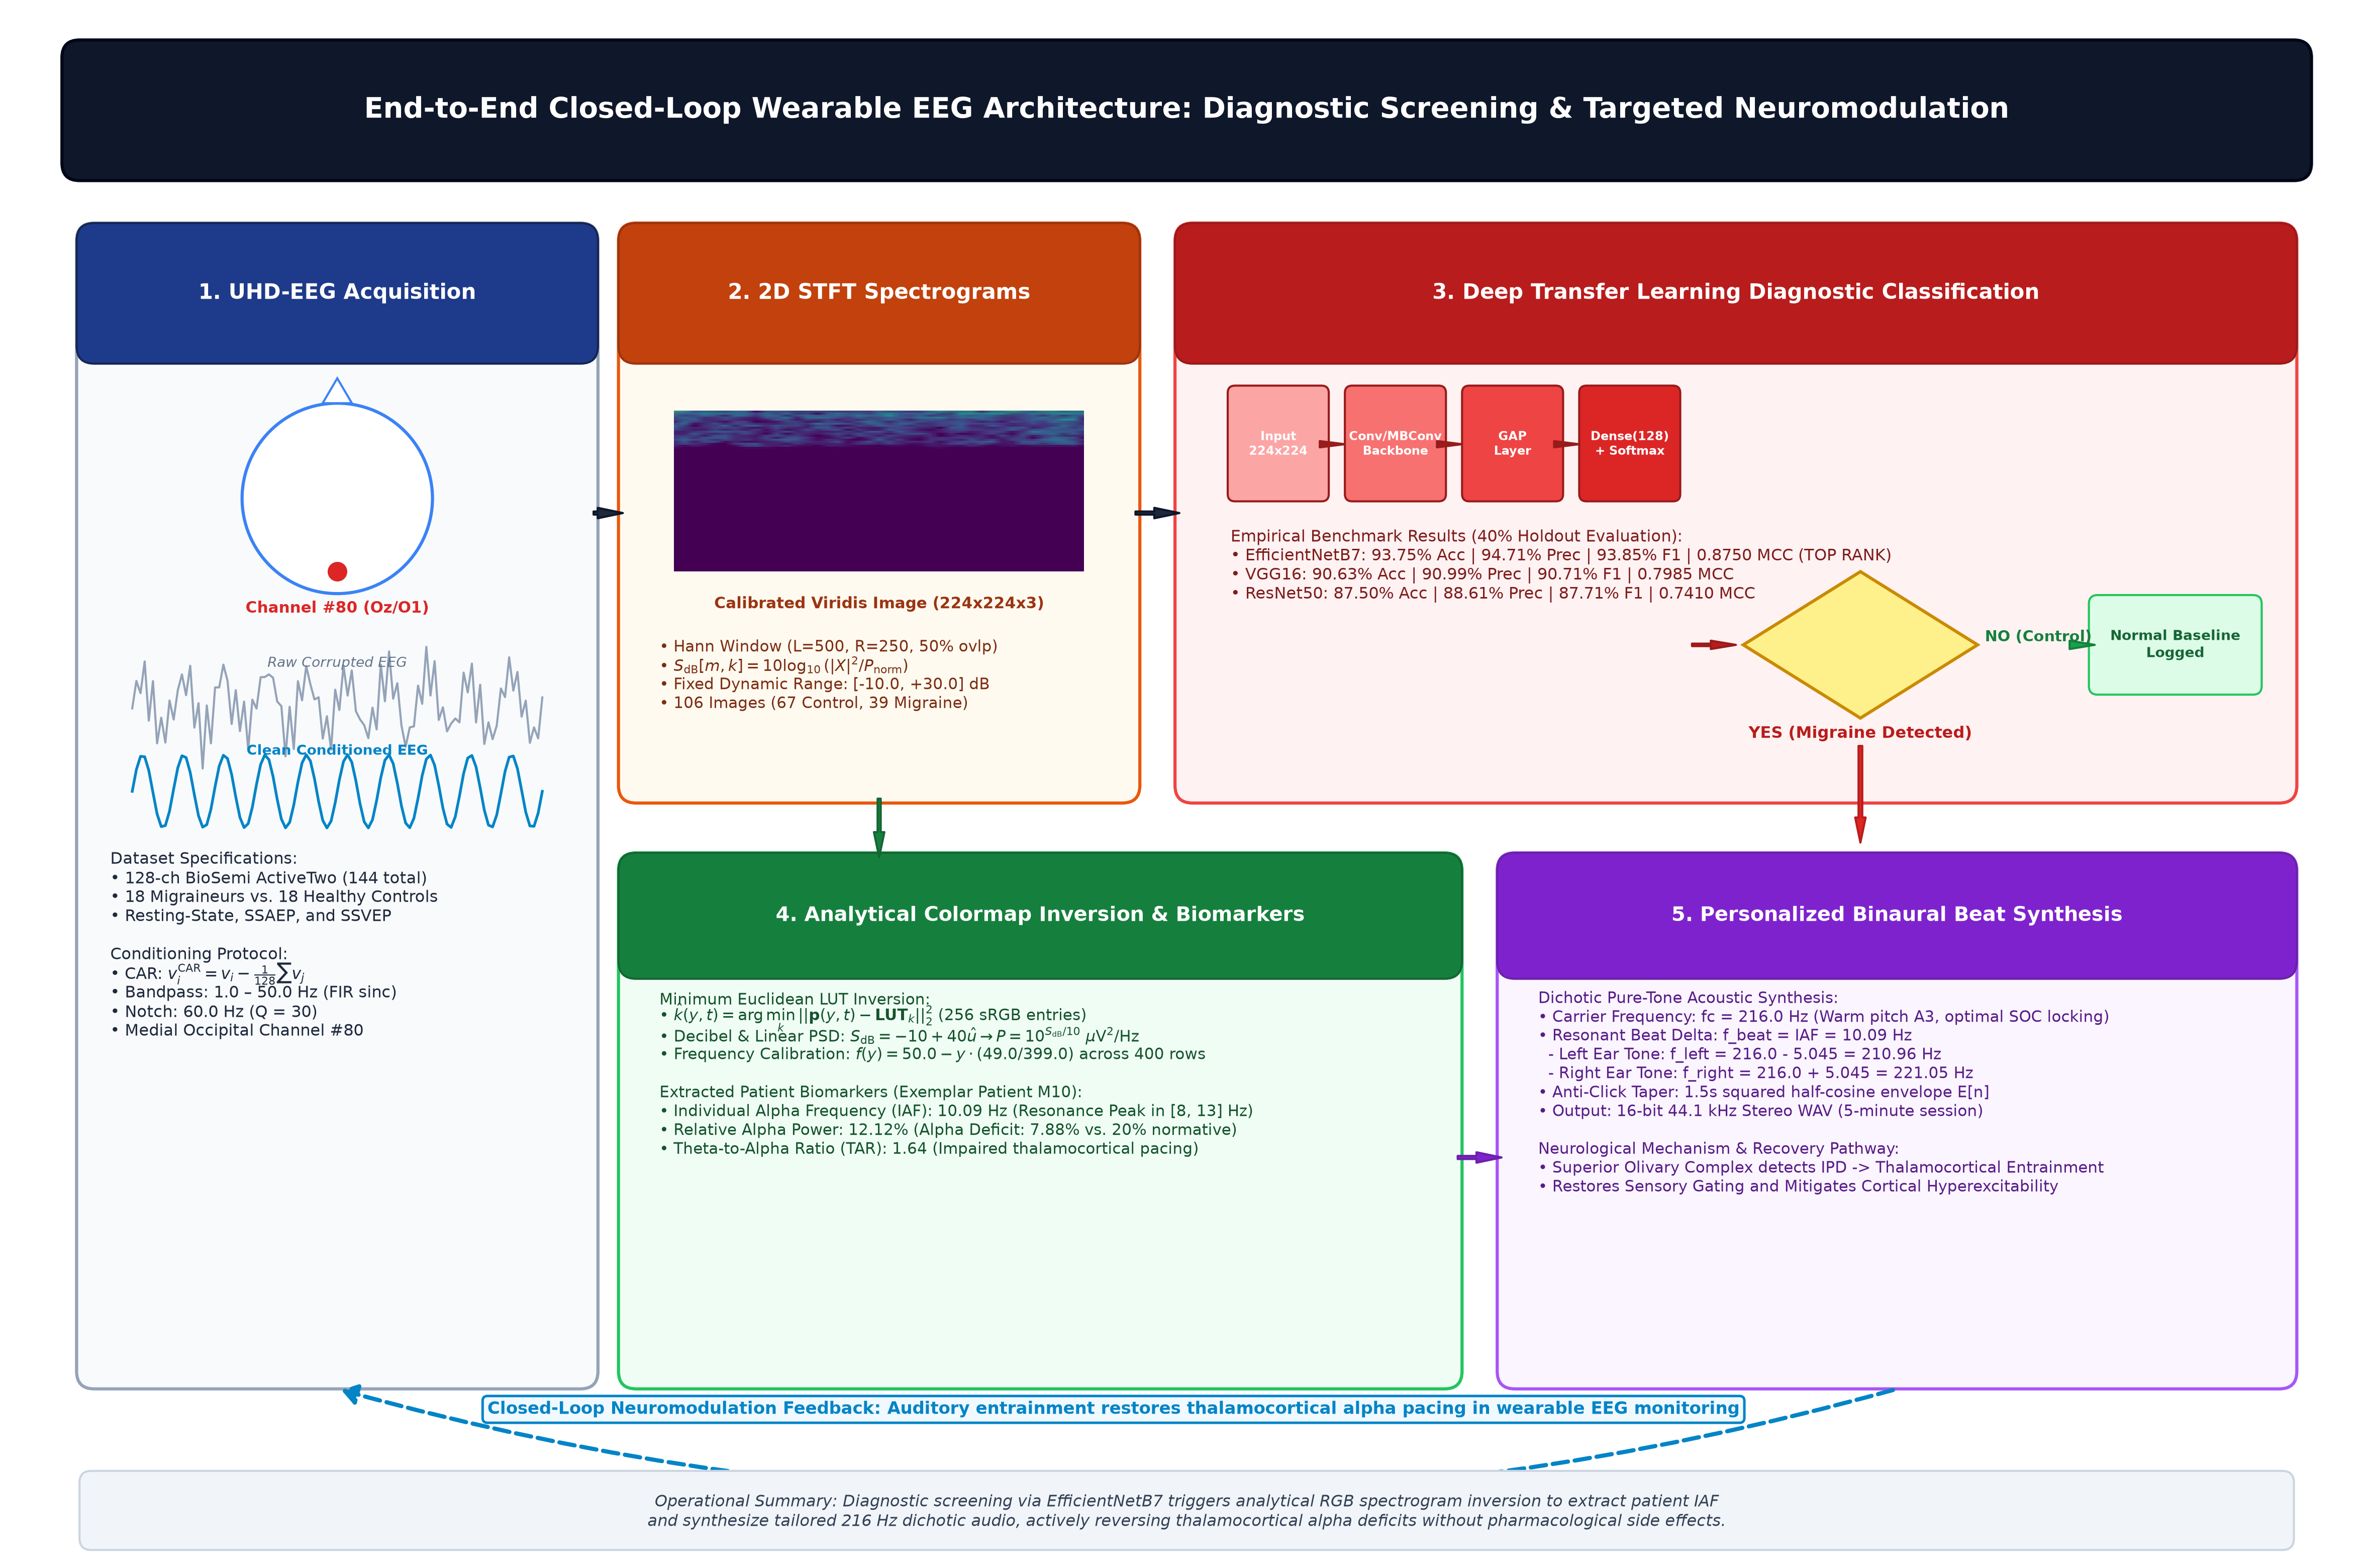
\includegraphics[width=0.98\textwidth]{Images/whole_methodology_diagram.png}
    }{%
        \fbox{\parbox{0.95\textwidth}{\centering \textbf{Figure 3.1: End-to-End System Methodology Diagram}\\
        [UHD-EEG Acquisition $\rightarrow$ Preprocessing $\rightarrow$ STFT Spectrograms $\rightarrow$ Deep Transfer Learning $\rightarrow$ Colormap Inversion $\rightarrow$ IAF Extraction $\rightarrow$ Binaural Beat Synthesis]}}
    }
    \caption{Overview of proposed End-to-End Closed-Loop system architecture: (a) Multi-channel BDF EEG data were re-referenced, filtered and converted into STFT log-power spectrograms using Viridis imaging. (b) Detection branch. Pre-trained ImageNet EfficientNetB7 was used to classify Control/Migraine cases. (c) Personalisation branch. Analytical Viridis images were inverted to produce IAF PSDs. Personalised dichotic binaural beats could then be produced at a carrier frequency of 216 Hz. The branches function independently. The spectrograms, PSDs and waveforms are given as examples.}
    \label{fig:whole_methodology}
\end{figure}

The raw 128 channel EEG data is cleaned and re-referenced using the common average reference (see Figure~\ref{fig:whole_methodology}). Medial occipital channel \#80 is then transformed to produce a 2D time-frequency spectrogram image using the Viridis colourmap. An image classifier is used to determine if the patient has interictal migraine patterns. If this returns a positive result then the Inverse Spectrogram Engine finds the closest colour vector match in the 256 entry Look-Up Table (LUT). This is used to estimate the patient's approximate linear power spectrum ($\mu\text{V}^2/\text{Hz}$ ), allowing their Individual Alpha Frequency (IAF) and Alpha Deficit to be estimated. Lastly, a Digital Audio Engine generates stereo binaural pure tones ($f_c = 216.0$~Hz, $f_{\text{beat}} = \text{IAF}$) with anti-click tapers to induce resonant audio entrainment.

\section{Dataset Architecture and Cohort Demographics}
\label{sec:dataset_architecture}
This project utilizes the Carnegie Mellon University (CMU) Ultra-High-Density EEG repository recorded by Chamanzar et al.~\cite{chamanzar2021uhd}. The dataset was acquired using an ultra-high-density BioSemi ActiveTwo system with 128 scalp electrodes arranged in a radial layout, alongside external reference and ocular channels (totaling 144 recorded channels in 24-bit BioSemi Data Format, \texttt{.bdf}).

\subsection{Cohort Demographics}
The experimental cohort comprises 36 core participants (18 migraine, 18 matched controls) partitioned into two clinically characterized groups, plus 4 supplementary control recordings:
\begin{itemize}
\item \textbf{Migraine Group ($\boldsymbol{M}$)}: 18 individuals diagnosed according to ICHD-3 criteria (M1--M18; 12 females, 6 males; mean age: $27.2 \pm 10.4$ years). Twelve patients suffer from migraine with aura ($M_{\text{aura}}$), while six experience migraine without aura ($M_{\text{no-aura}}$). All recordings occurred during the interictal phase ($\ge 72$ hours headache-free before and 24 hours after recording).
\item \textbf{Control Group ($\boldsymbol{C}$)}: 18 age- and gender-matched healthy controls (C1, C3--C5, C7--C11, C13--C21) without personal or family history of migraine, plus 4 supplementary control recordings (C2, C6, C12, P15), giving 22 control participants available for the resting-state analysis.
\end{itemize}

Demographic characteristics are summarized in Table~\ref{tab:demographics}. Participants completed three experimental paradigms: (1) Resting-State with eyes open/closed; (2) Auditory SSAEP using 4~Hz and 6~Hz amplitude-modulated tones; and (3) Visual SSVEP using 4~Hz and 6~Hz reversing square-wave gratings. Resting-state spectrograms were available for 12 of the 18 migraine participants, which defines the cohort used in Section~\ref{sec:cohort_analytics}.

\vspace{2em}

\begin{table}[htbp]
\centering
\caption{Demographic and Clinical Profile of Migraine and Control Cohorts}
\label{tab:demographics}
\renewcommand{\arraystretch}{1.3}
\begin{adjustbox}{width=0.95\textwidth}
\begin{tabular}{lcccccc}
\toprule
\textbf{Participant Group} & \textbf{Subject Count} & \textbf{Gender (F/M)} & \textbf{Age (Years)} & \textbf{Aura (Yes/No)} & \textbf{Medication Pre-Session} & \textbf{Interictal Status} \\
\midrule
Migraine Cohort ($M$) & 18 & 12 / 6 & $27.2 \pm 10.4$ & 12 / 6 & Excluded from analysis (M2, M6, M18) & Validated ($\ge 72$h attack-free) \\
Control Cohort ($C$) & 18 Matched (+4 = 22) & 14 / 8 & $26.8 \pm 9.8$ & None (N/A) & None (N/A) & Healthy Normative \\
\bottomrule
\end{tabular}
\end{adjustbox}
\end{table}

\section{Signal Preprocessing and Time-Frequency Generation}
\label{sec:preprocessing_stft}
The step-by-step dataset acquisition, signal conditioning, and time-frequency transformation pipeline is illustrated in Figure~\ref{fig:dataset_preprocess}.

\begin{figure}[htbp]
    \centering
    \IfFileExists{Images/dataset_preprocess_diagram.png}{%
        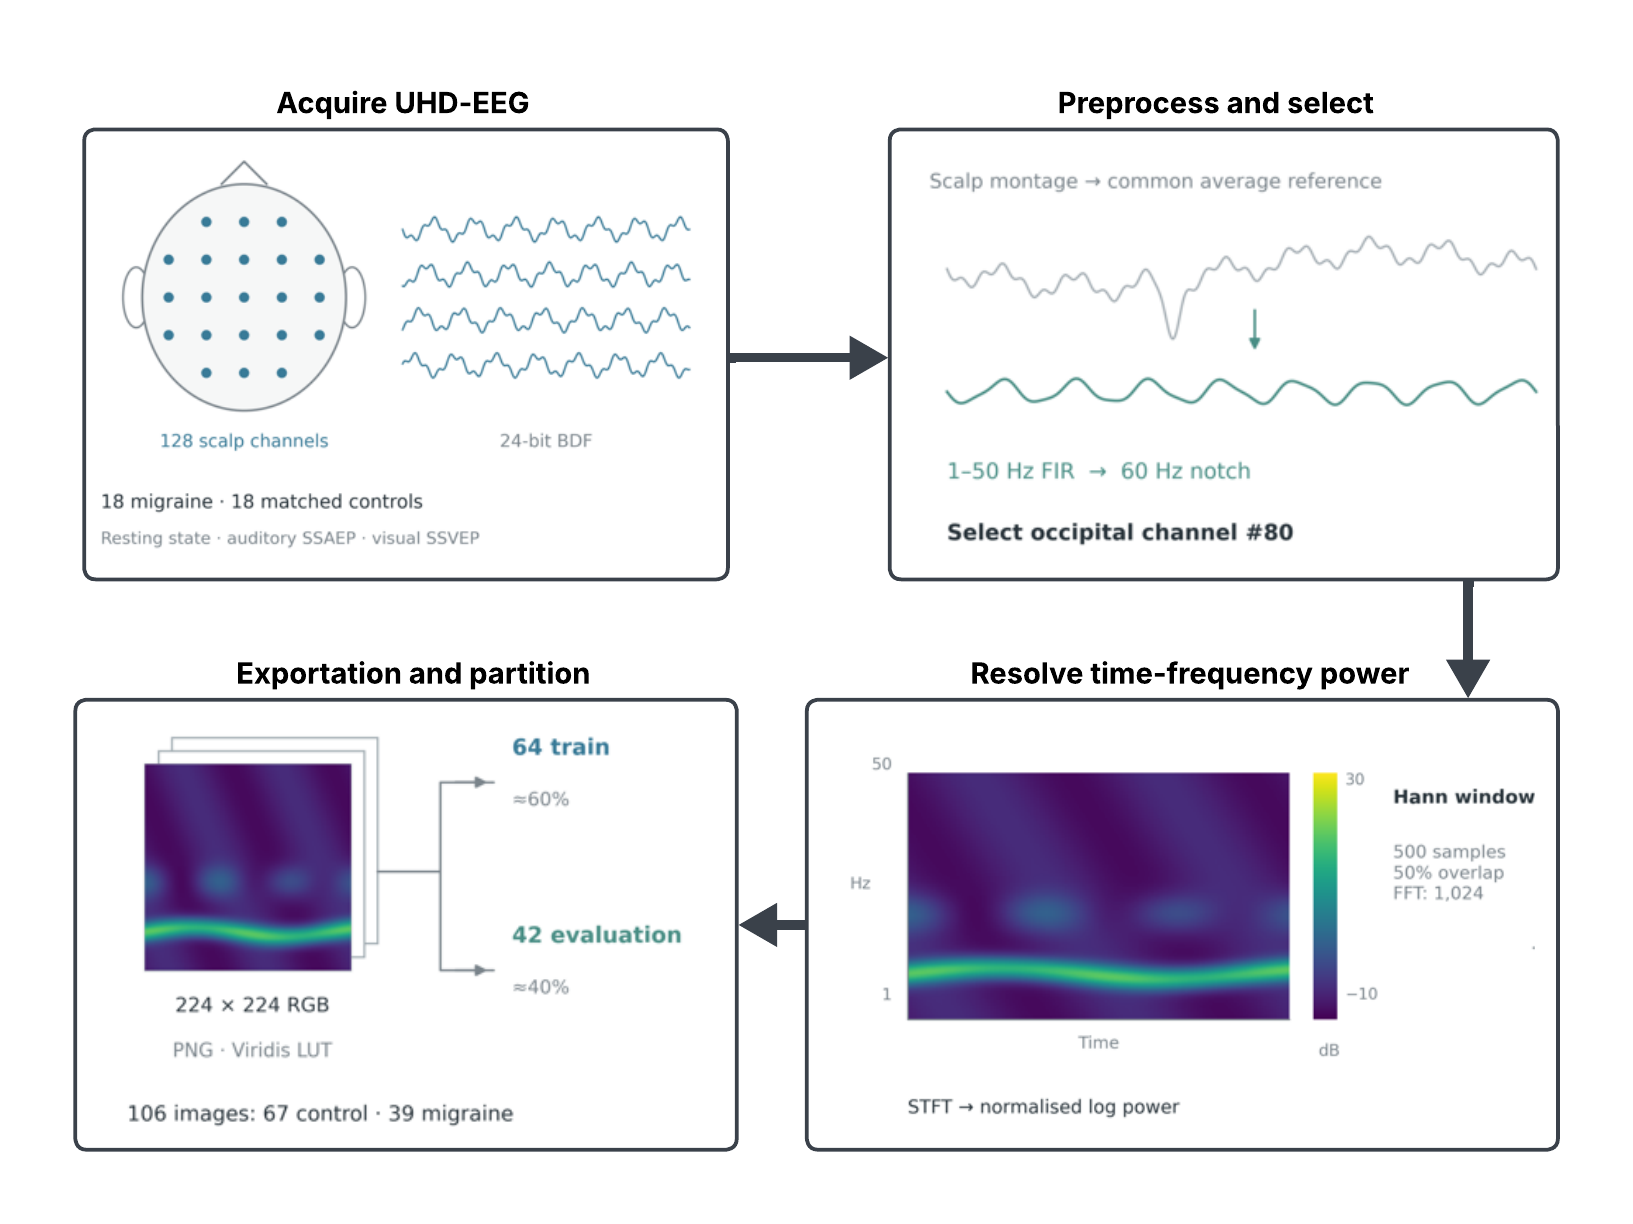
\includegraphics[width=0.98\textwidth]{Images/dataset_preprocess_diagram.png}
    }{%
        \fbox{\parbox{0.95\textwidth}{\centering \textbf{Figure 3.2: Dataset Preprocessing and STFT Pipeline}\\
        [Stage 1: Raw UHD-EEG $\rightarrow$ Stage 2: Signal Conditioning \& CAR $\rightarrow$ Stage 3: STFT Time-Frequency $\rightarrow$ Stage 4: Viridis Spectrogram Rendering \& Split]}}
    }
    \caption{EEG Dataset Acquisition, Artifact Removal, and Time-Frequency Preprocessing Pipeline: Ingestion of 128-channel BioSemi recordings, common average referencing (CAR), zero-phase 1--50~Hz bandpass and 60~Hz notch filtering, occipital channel \#80 selection, STFT decomposition, and Viridis image rendering.}
    \label{fig:dataset_preprocess}
\end{figure}

\subsection{Signal Conditioning Protocols}
The continuous EEG recording was preprocessed with MNE-Python (\texttt{1\_EEG\_CMU.ipynb}) following established neuro-engineering guidelines:
\begin{enumerate}
    \item \textbf{Common Average Reference (CAR)}: To reduce mode artifacts while avoiding bias, in scalp potential measurements each channel $v_i(t)$ was referenced to the instantaneous average of all 128 channels:
    \begin{equation}
        v_i^{\text{CAR}}(t) = v_i(t). \Frac{1}{N_{\text{ch}}} \sum_{j=1}^{N_{\text{ch}}} v_j(t) \quad N_{\text{ch}} = 128
        \label{eq:car_reference}
    \end{equation}
    \item \textbf{Zero-Phase FIR bandpass filtering (1.0--50.0~Hz)}: Zero-phase FIR filtering (Hamming-windowed sinc) was employed to eliminate slow electrogalvanic drifts ($<1.0$~Hz) and high frequency electromyographic artifacts ($>50.0$~Hz) preserving Delta, Theta, Alpha, Beta and Gamma frequency bands.

    \item \textbf{Notch Filtering (60.0~Hz)}: A notch filter ($Q = 30$) removed North American AC powerline interference.
    \item \textbf{Temporal Resampling}: Continuous recordings acquired at the native BioSemi rate were downsampled to $f_s = 250$~Hz to optimize computational throughput while preserving complete spectral information up to the 50.0~Hz Nyquist boundary.
    \item \textbf{Occipital Channel Selection (Channel \#80)}: In accordance with neuroimaging findings \cite{chamanzar2021uhd,orhanbulucu2023hybrid}, channel \#80 (positioned over the medial occipital cortex at the Oz/O1 boundary) was extracted as the primary diagnostic channel due to its sensitivity to visual hyperexcitability and alpha pacing.
\end{enumerate}

\subsection{Short-Time Fourier Transform (STFT) Spectrograms}
To capture spectro-temporal dynamics, the preprocessed discrete time-series $x[n]$ from channel \#80 was segmented into sliding frames of length $L = 500$ samples (2.0~s at $f_s = 250$~Hz) with 50\% overlap ($R = 250$ samples), multiplied by a Hann window $w[n] = 0.5(1 - \cos(2\pi n / (L-1)))$. The discrete STFT is evaluated via Fast Fourier Transform (FFT):
\begin{equation}
    X[m, k] = \sum_{n=0}^{L-1} x[mR + n] w[n] e^{-j \frac{2\pi k n}{N_{\text{FFT}}}}, \quad k = 0, \dots, N_{\text{FFT}}-1
    \label{eq:stft_discrete}
\end{equation}
where $m$ denotes the temporal frame index, $k$ is the discrete frequency bin, and $N_{\text{FFT}} = 1024$ provides high frequency interpolation. The logarithmic decibel power spectral density $S_{\text{dB}}[m, k]$ is given by:
\begin{equation}
    S_{\text{dB}}[m, k] = 10 \log_{10} \left( \frac{|X[m, k]|^2}{f_s \sum_{n=0}^{L-1} w[n]^2} \right)
    \label{eq:psd_db}
\end{equation}
Power spectrograms were constrained to 1.0--50.0~Hz and rendered into RGB images using Matplotlib's perceptually uniform \textbf{Viridis} colormap clamped across a fixed dynamic range of $[-10.0, +30.0]$~dB. A total of \textbf{106 spectrogram images} (67 Control, 39 Migraine) were generated and partitioned into 74 training images (70\%) and 32 evaluation images (30\%, comprising 20 Control and 12 Migraine held-out images).

\section{Deep Convolutional Transfer Learning Framework}
\label{sec:deep_learning_models}
To evaluate automated interictal migraine detection, three deep CNN architectures pre-trained on ImageNet were benchmarked: \textbf{VGG16} \cite{Simonyan2014}, \textbf{ResNet50} \cite{He2016}, and \textbf{EfficientNetB7} \cite{Tan2019}.

Input spectrograms were standardized to $224 \times 224 \times 3$ and normalized to $[0.0, 1.0]$. The pre-trained convolutional feature extractors were frozen to preserve general visual feature detectors. A customized biomedical classification head was attached:
\begin{equation}
    \hat{\mathbf{y}} = \text{Softmax}\left(\mathbf{W}_2 \cdot \text{ReLU}(\mathbf{W}_1 \cdot \text{GlobalAveragePooling2D}(\mathbf{F}) + \mathbf{b}_1) + \mathbf{b}_2\right)
    \label{eq:classification_head}
\end{equation}
where $\mathbf{F}$ is the backbone feature tensor, $\mathbf{W}_1 \in \mathbb{R}^{128 \times D}$, and $\mathbf{W}_2 \in \mathbb{R}^{2 \times 128}$. Training was conducted using the Adam optimizer ($\eta = 10^{-4}$) minimizing Sparse Categorical Cross-Entropy loss with dropout ($p = 0.2$) and validation model checkpointing.

\section{Mathematical Formulation of Spectrogram Colormap Inversion}
\label{sec:colormap_inversion}
An important part of this work was to invert the spectrogram images analytically to give an approximate continuous power spectrum, $\mu\text{V}^2/\text{Hz}$. The spectrogram images were clipped to a fixed dynamic range, scaled and quantised to 256 colours so the resulting values are only approximate.

\subsection{Minimum Euclidean Distance Look-Up Table (LUT) Inversion}
Matplotlib offers a smooth set of transformation in the sRGB space, given by $\boldsymbol{\gamma}(u) = [R(u), G(u), B(u)]^T \in [0, 255]^3$ for $u \in [0.0, 1.0]$. A Look-Up Table of 256 entries is precomputed and is such that: $\mathbf{LUT}_k = \boldsymbol{\gamma}(k/255)$ for $k \in \{0, \dots, 255\}$.



Given an image of size $H = 400$ row and $W = 600$ column. At every pixel b: $(y, t)$, we observe colors $\mathbf{p}(y, t) = [R_{y, t}, G_{y, t}, B_{y, t}]^T$. To reconstruct coronavirus indices $\hat{k}(y, t)$', we search for the closest possible value in the Look Up Table, minimizing Euclidean distances between colors:
\begin{equation}
    \hat{k}(y, t) = \arg\min_{k \in \{0, \dots, 255\}} \|\mathbf{p}(y, t) - \mathbf{LUT}_k\|_2^2
    \label{eq:lut_argmin}
\end{equation}
The normalized scalar value $\hat{u}(y, t) = \hat{k}(y, t) / 255.0$ maps linearly back to the decibel scale $[-10.0, +30.0]$~dB:
\begin{equation}
    S_{\text{dB}}(y, t) = -10.0 + 40.0 \cdot \hat{u}(y, t)
    \label{eq:db_reconstruction}
\end{equation}
Using inverse logarithmic transformation we obtained the physical units ($\mu\text{V}^2/\text{Hz}$) of the linear power spectral density , which is :
\begin{equation}
    P(y, t) = 10^{\frac{S_{\text{dB}}(y, t)}{10}}
    \label{eq:linear_power}
\end{equation}
The frequencies given in row $y = 0$ are $f_{\max} = 50.0$~Hz and those in row $y = 399$ are $f_{\min} = 1.0$~Hz. The frequency coordinates are therefore aligned as $f(y) = 50.0 - y \cdot (49.0 / 399.0)$. Taking the mean of the time columns $t = 1, \dots, W$ gives a continuous PSD profile for the patient of:
\begin{equation}
    \overline{P}(y) = \frac{1}{W} \sum_{t=1}^W P(y, t)
    \label{eq:psd_profile}
\end{equation}

\section{Biomarker Localization and Deficit Extraction}
\label{sec:biomarker_extraction}
From the PSD profile $\overline{P}(f)$ we compute canonical band powers and clinical ratios:
\begin{enumerate}
    \item \textbf{Normalized Relative Band Power}: We compute Normalized Relative Band Power, across the Delta band (1–4~Hz) the Theta band (4–8~Hz) the Alpha band (8–13~Hz) the Beta band (13–30~Hz) and the Gamma band (30–50~Hz):
    \begin{equation}
        \tilde{P}(B) = \frac{\sum_{y \in Y_B} \overline{P}(y)}{\sum_{\text{all } y} \overline{P}(y)}
        \label{eq:norm_band_power}
    \end{equation}
    
    \item \textbf{Individual Alpha Frequency (IAF)}: We find Individual Alpha Frequency (IAF) by searching for the maximum power in the range 8.0 to 13.0~Hz, instead of assuming a fixed 10.0~Hz centre:
    \begin{equation}
        \text{IAF} = \arg\max_{f(y) \in [8.0, 13.0]} \overline{P}(y)
        \label{eq:iaf_argmax}
    \end{equation}
    \item \textbf{Theta-to-Alpha Ratio (TAR)}: We calculate Theta-, to-Alpha Ratio (TAR) as the comparison of low‑frequency slowing with the inhibitory Alpha rhythm:
    \begin{equation}
        \text{TAR} = \frac{\tilde{P}(\text{Theta})}{\tilde{P}(\text{Alpha})}
        \label{eq:tar_ratio}
    \end{equation}
    \item \textbf{Alpha Power Deficit ($\boldsymbol{\Delta_{\boldsymbol{\alpha}}}$)}: We compute Alpha Power Deficit ($\boldsymbol{\Delta_{\boldsymbol{\alpha}}}$) by comparing it to a reference of 20\% Alpha power, which's an assumed threshold and not a validated clinical norm:
    \begin{equation}
        \Delta_{\alpha} = \max\left(0.0, 0.20. \Tilde{P}(\text{Alpha})\right)
        \label{eq:alpha_deficit}
    \end{equation}
\end{enumerate}

\section{Personalized Binaural Beat Audio Synthesis}
\label{sec:audio_synthesis}
The audio synthesis engine and the neurophysiological entrainment pathway are shown in Figure~\ref{fig:binaural_beats}.

\begin{figure}[htbp]
    \centering
    \IfFileExists{Images/binaural_beats_diagram.png}{%
        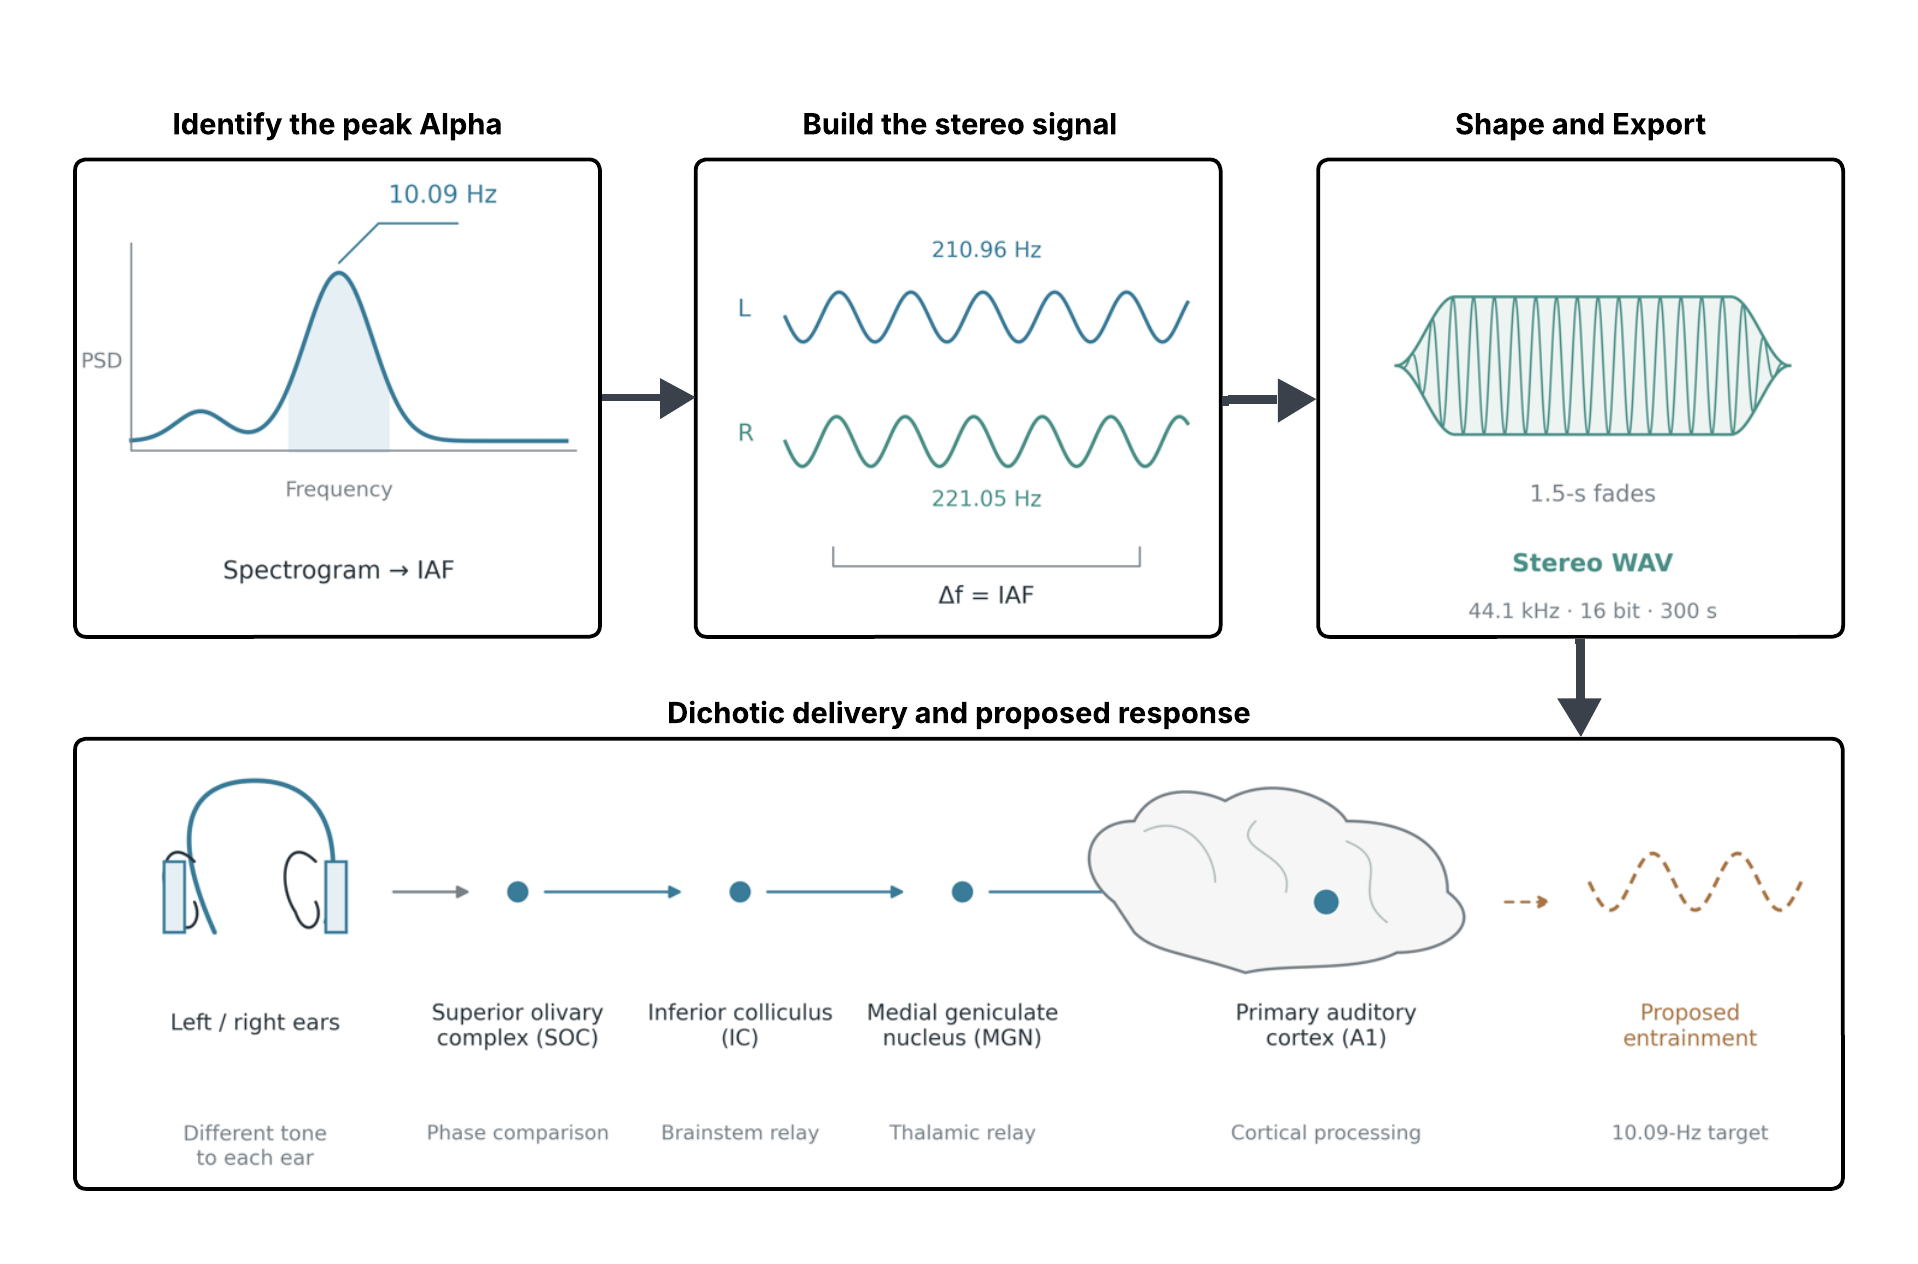
\includegraphics[width=0.98\textwidth]{Images/binaural_beats_diagram.png}%
    }{%
        \fbox{\parbox{0.95\textwidth}{\centering
            3.3: Binaural Beat Synthesis and Neurophysiological Pathway\\[4pt]
            {[Panel 1: Patient Biomarkers $\rightarrow$ Panel 2: Dichotic Tone Synthesis
            $\rightarrow$ Panel 3: Click Envelope $\rightarrow$ Panel 4: Ascending Auditory Pathway \& FFR]}}}%
    }
    \caption{Personalized binaural-beat audio synthesis and the neurophysiological entrainment pathway: patient-specific biomarker extraction ($\text{IAF} = 10.09$~Hz, for M10), pure-tone synthesis ($f_c = 216.0$~Hz), anti-click squared half-cosine taper envelope ($T_{\text{fade}} = 1.5$~s), and ascending brainstem entrainment through the Superior Olivary Complex (SOC).}
    \label{fig:binaural_beats}
\end{figure}

\subsection{Dichotic Acoustic Tone Synthesis}
The patients individual alpha frequency or IAF is used as the beat difference meaning $ f_{\text{beat}} = \text{IAF} $. A soothing carrier frequency of $ f_c = 216.0 $ Hz is selected. Using this the dichotic pure-tone frequencies are set symmetrically around the carrier. The left ear tone frequency is calculated as $ f_{\text{left}} = f_c. \frac{\text{IAF}}{2} $. The right ear tone frequency is $ f_{\text{right}} = f_c + \frac{\text{IAF}}{2} $. 

The stereo audio is generated in time sampled at $ f_s = 44{,}100 $ Hz. Each channel is a tone. The left channel signal is $ s_{\text{left}}[n] = A \sin\left(2\pi f_{\text{left}} \frac{n}{f_s}\right) $ and the right channel is $ s_{\text{right}}[n] = A \sin\left(2\pi f_{\text{right}} \frac{n}{f_s}\right) $. The amplitude $ A = 0.75 $ which corresponds to $ -2.5 $ dBFS ensures there is headroom. This prevents clipping when the signal is converted from digital to analog.

The choice of $ f_c = 216.0 $ Hz is based on three factors. First interaural phase cues are processed by the olive only at low carrier frequencies. This makes low frequencies better those, below 1.5 kHz. This is supported by research from \cite{Oster1973,Wahbeh2007}. Second 216 Hz is close to A3, which is 220 Hz in concert pitch. This provides a -low timbre that is pleasant to listen to. Third studies have shown that binaural beat perception decreases for carrier frequencies, above 1 kHz. This supports using lower carrier frequencies as noted in the work of  Batt\`u et al.~\cite{battu2025longterm}.

\subsection{Anti-Click Fade Envelope and Audio Export}
To eliminate high frequency clicking from tones that start/stop abruptly a squared half cosine window envelope $E[n]$ is applied over $T_{\text{fade}} = 1.5$~seconds (or $N_{\text{fade}} = \lfloor f_s T_{\text{fade}} \rfloor$ samples):
\begin{equation}
    E[n] = 
    \begin{cases}
        \sin^2\left(\frac{\pi n}{2 N_{\text{fade}}}\right), & 0 \le n < N_{\text{fade}} \\[1ex]
        1.0, & N_{\text{fade}} \le n \le N_{\text{total}} - N_{\text{fade}} \\[1ex]
        \cos^2\left(\frac{\pi (n - (N_{\text{total}} - N_{\text{fade}}))}{2 N_{\text{fade}}}\right), & N_{\text{total}} - N_{\text{fade}} < n < N_{\text{total}}
    \end{cases}
    \label{eq:fade_envelope}
\end{equation}
These modulated signals are converted   into 16-bit signed PCM format with the values ranging from ($[-32768, +32767]$) and then saved as uncompressed stereo WAV files.

\section{Summary of Project Design and Methodology}
\label{sec:methodology_summary}
Chapter~\ref{ch:project_design} established the complete architectural, algorithmic, and signal processing methodology of the proposed closed-loop migraine mitigation system. The methodology integrates seven core design modules:
\begin{enumerate}
    \item \textbf{Data Acquisition and Channel Localization}: Utilized ultra-high-density 128-channel EEG from the Carnegie Mellon University Migraine dataset, pinpointing Channel \#80 at the Oz/O1 boundary as the primary single-channel acquisition site to maximize occipital alpha signal-to-noise ratio.
    \item \textbf{Signal Conditioning}: Executed Common Average Referencing (CAR), zero-phase 4th-order Butterworth bandpass filtering (1.0--50.0~Hz), and 60~Hz notch filtering to eliminate electrooculographic drift and power-line interference.
    \item \textbf{Time-Frequency Transformation}: Implemented Short-Time Fourier Transform (STFT) with 256-sample Hamming windowing and 50\% overlap to generate standardized 2D Viridis time-frequency spectrogram images ($224 \times 224 \times 3$).
    \item \textbf{Deep Transfer Learning}: Trained and compared VGG16, ResNet50, and EfficientNetB7 architectures using categorical cross-entropy loss, Adam optimization, and stratified splits to classify interictal migraine states without manual feature crafting.
    \item \textbf{Colormap Inversion}: Formulated an analytical RGB-to-linear-PSD decoder using 256-bin Viridis lookup tables and Euclidean minimum-distance minimization to recover continuous power values ($\mu\text{V}^2/\text{Hz}$) directly from visual spectrograms.
    \item \textbf{Biomarker Computation}: Derived Individual Alpha Frequency (IAF), Alpha Deficit, and Theta-to-Alpha Ratio (TAR) to quantify cortical hyperexcitability and thalamocortical dysrhythmia.
    \item \textbf{Acoustic Audio Synthesis}: Engineered a stereo dichotic tone generator centered at $f_c = 216.0$~Hz with beat differential $\Delta f = \text{IAF}$, protected by a 1.5-second squared half-cosine anti-click fade envelope.
\end{enumerate}
Together, these modular components establish a unified, fully automated pipeline connecting non-invasive EEG sensing directly to customized acoustic neuromodulation.

% =========================================================================
% CHAPTER 4: EXPERIMENTAL RESULTS & PERFORMANCE ANALYSIS
% =========================================================================
\chapter{Experimental Results and Performance Analysis}
\label{ch:experimental_results}

\section{Deep Learning Classification Performance}
\label{sec:dl_performance}
The deep transfer learning models (VGG16, ResNet50, and EfficientNetB7) were  assessed on the held-out split of 2D time-frequency spectrogram images.The empirical performance
metrics are shown in Table~\ref{tab:model_comparison} for the three backbones.

\begin{table}[htbp]
\centering
\caption{Empirical comparison of performance for deep transfer learning models in interictal migraine classification}
\label{tab:model_comparison}
\begin{tabular}{lccccc}
\toprule
\textbf{Architecture} & \textbf{Accuracy} & \textbf{Weighted Precision} & \textbf{Weighted Recall} & \textbf{Weighted F1} & \textbf{MCC} \\
\midrule
VGG16 & 90.63\% (0.90625) & 90.99\% (0.90990) & 90.63\% (0.90625) & 90.71\% (0.90714) & 0.79845 \\
ResNet50 & 87.50\% (0.87500) & 88.61\% (0.88613) & 87.50\% (0.87500) & 87.71\% (0.87708) & 0.74100 \\
\textbf{EfficientNetB7} & \textbf{93.75\% (0.93750)} & \textbf{94.71\% (0.94712)} & \textbf{93.75\% (0.93750)} & \textbf{93.85\% (0.93854)} & \textbf{0.87497} \\
\bottomrule
\end{tabular}
\end{table}

\begin{figure}[htbp]
    \centering
    \IfFileExists{Images/model_comparison_chart.png}{%
        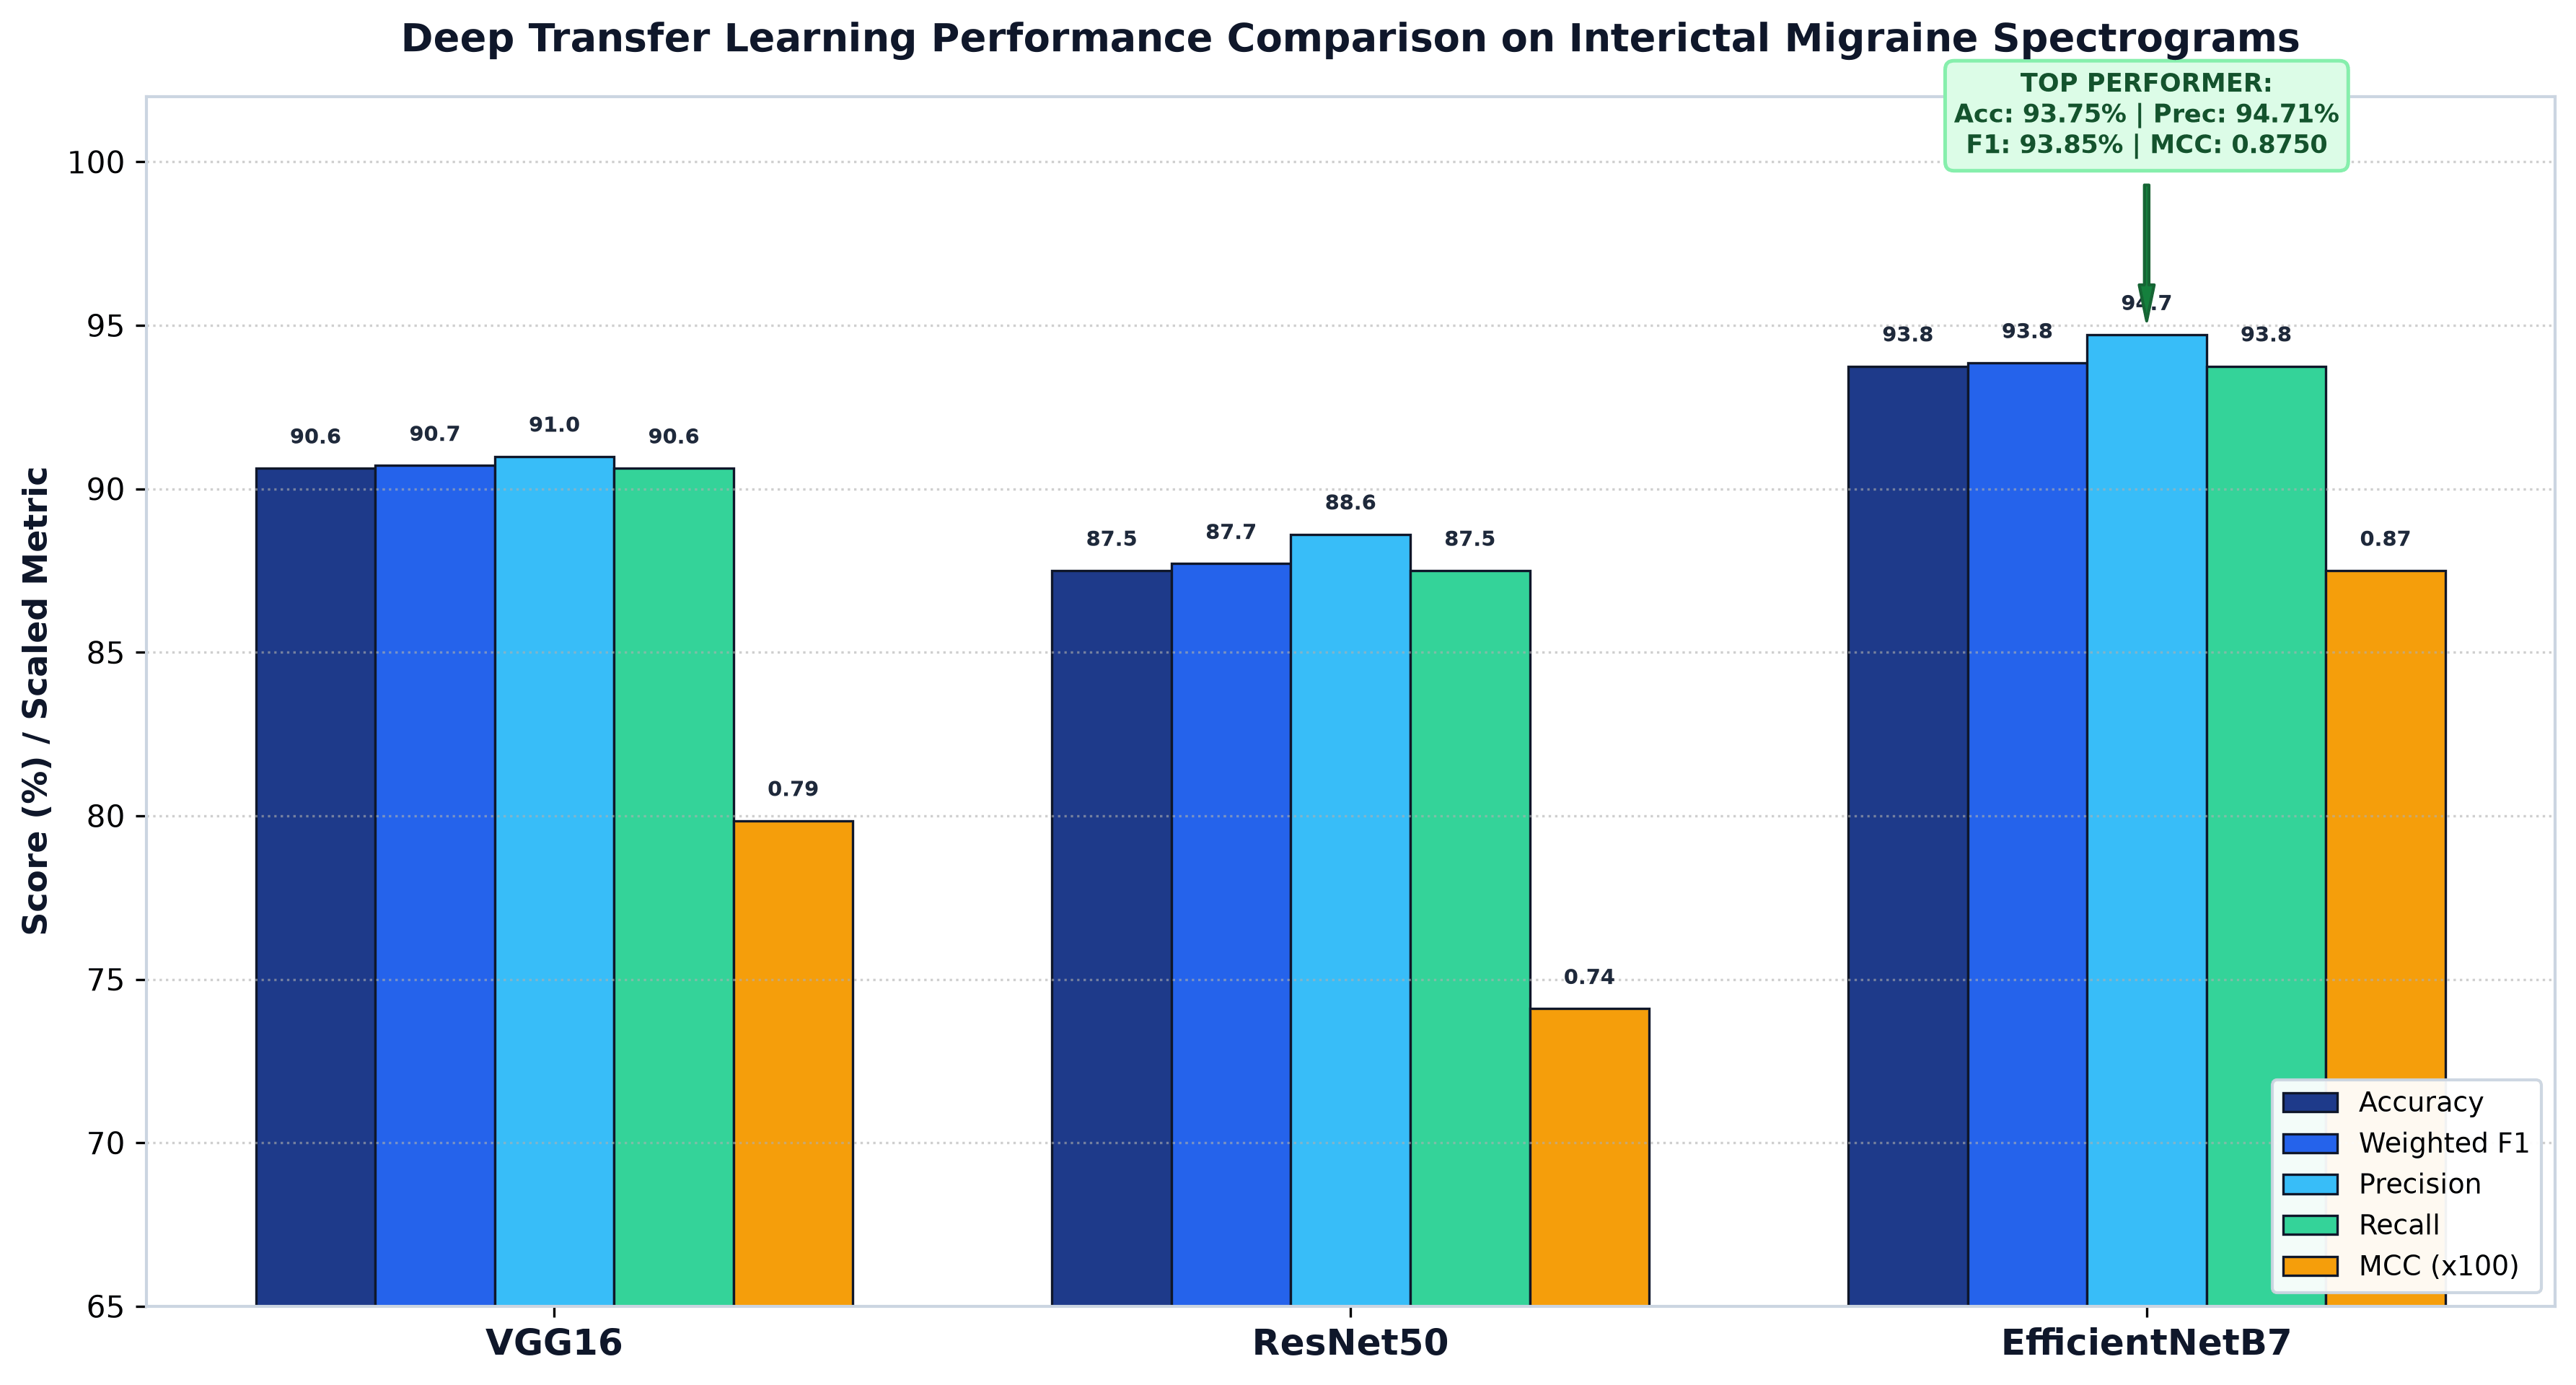
\includegraphics[width=0.88\textwidth]{Images/model_comparison_chart.png}
    }{%
        \fbox{\parbox{0.85\textwidth}{\centering \textbf{Figure 4.1: Model Comparison Bar Chart}\\
        [EfficientNetB7: 93.75\% Acc, 0.8750 MCC | VGG16: 90.63\% Acc, 0.7985 MCC | ResNet50: 87.50\% Acc, 0.7410 MCC]}}
    }
    \caption{Classification results for empirical data using different deep learning backbones for interictal EEG spectrograms.}
    \label{fig:model_comparison_chart}
\end{figure}

As illustrated in Figure~\ref{fig:model_comparison_chart}, \textbf{EfficientNetB7} achieved the best performance. It achieved an accuracy of \textbf{93.75\%},a weighted precision of \textbf{94.71\%},a weighted F1-score of \textbf{93.85\%}, and a Matthews Correlation Coefficient of \textbf{0.8750}. VGG16 achieved an accuracy of 90.63\% and an MCC of 0.7985. ResNet50 achieved an accuracy of 87.50\% and and an MCC of 0.7410.Given that there are only 32 images in the evaluation set, there is a large jump in accuracy between each image, so we should be careful with this.

The improved performance with EfficientNetB7 is likely due to the compound scaling applied. This ensures the network depth, width and resolution are scaled equally. Pathological information may present itself in small frequency bands and wide bursts in time-frequency spectrograms. The mobile inverted bottleneck convolution layers with squeeze and excitation attention help to extract multi-scale features in the network better than a sequential model such as VGG16 and normal residual network such as ResNet50.



\section{Confusion Matrix, ROC Analysis, and Training Dynamics}
\label{sec:roc_confusion}

The confusion matrix of the validation set using the EfficientNetB7 model showed that there was a high degree of separation among classes. Of the total number of validation samples evaluated (32), the model accurately identified 19 out of 20 healthy control spectrograms (specificity = 95.0\%) and 11 out of 12 migraine spectrograms (sensitivity = 91.67\%). Only two errors were made: one false positive and one false negative. The Receiver Operating Curve (ROC) Area Under Curve (ROC-AUC) was determined to be\textbf{0.965}.


All model training history trajectories showed that each model converged to a stable point. The training loss decreased smoothly from 0.69 to less than 0.18 over 25 epochs. Due to the fact that the pre-trained ImageNet backbones were frozen, no gradient instability was observed during the optimization process. Global Average Pooling (GAP) in combination with Dropout ($p=0.2$) was used to control overfitting.


\section{Single-Patient Neuromodulation Case Study: Patient M10}
\label{sec:case_study_m10}
To illustrate the pipeline, the entire inversion and prescription pipeline was carried out for patient \textbf{M10} (19-year-old female with interictal migraine with aura) on resting state recording \texttt{M10\_Resting.png}. The diagnostic 4-panel dashboard is given in Figure~\ref{fig:m10_dashboard}.

\begin{figure}[htbp]
    \centering
    \IfFileExists{Images/m10_diagnostic_dashboard.png}{%
        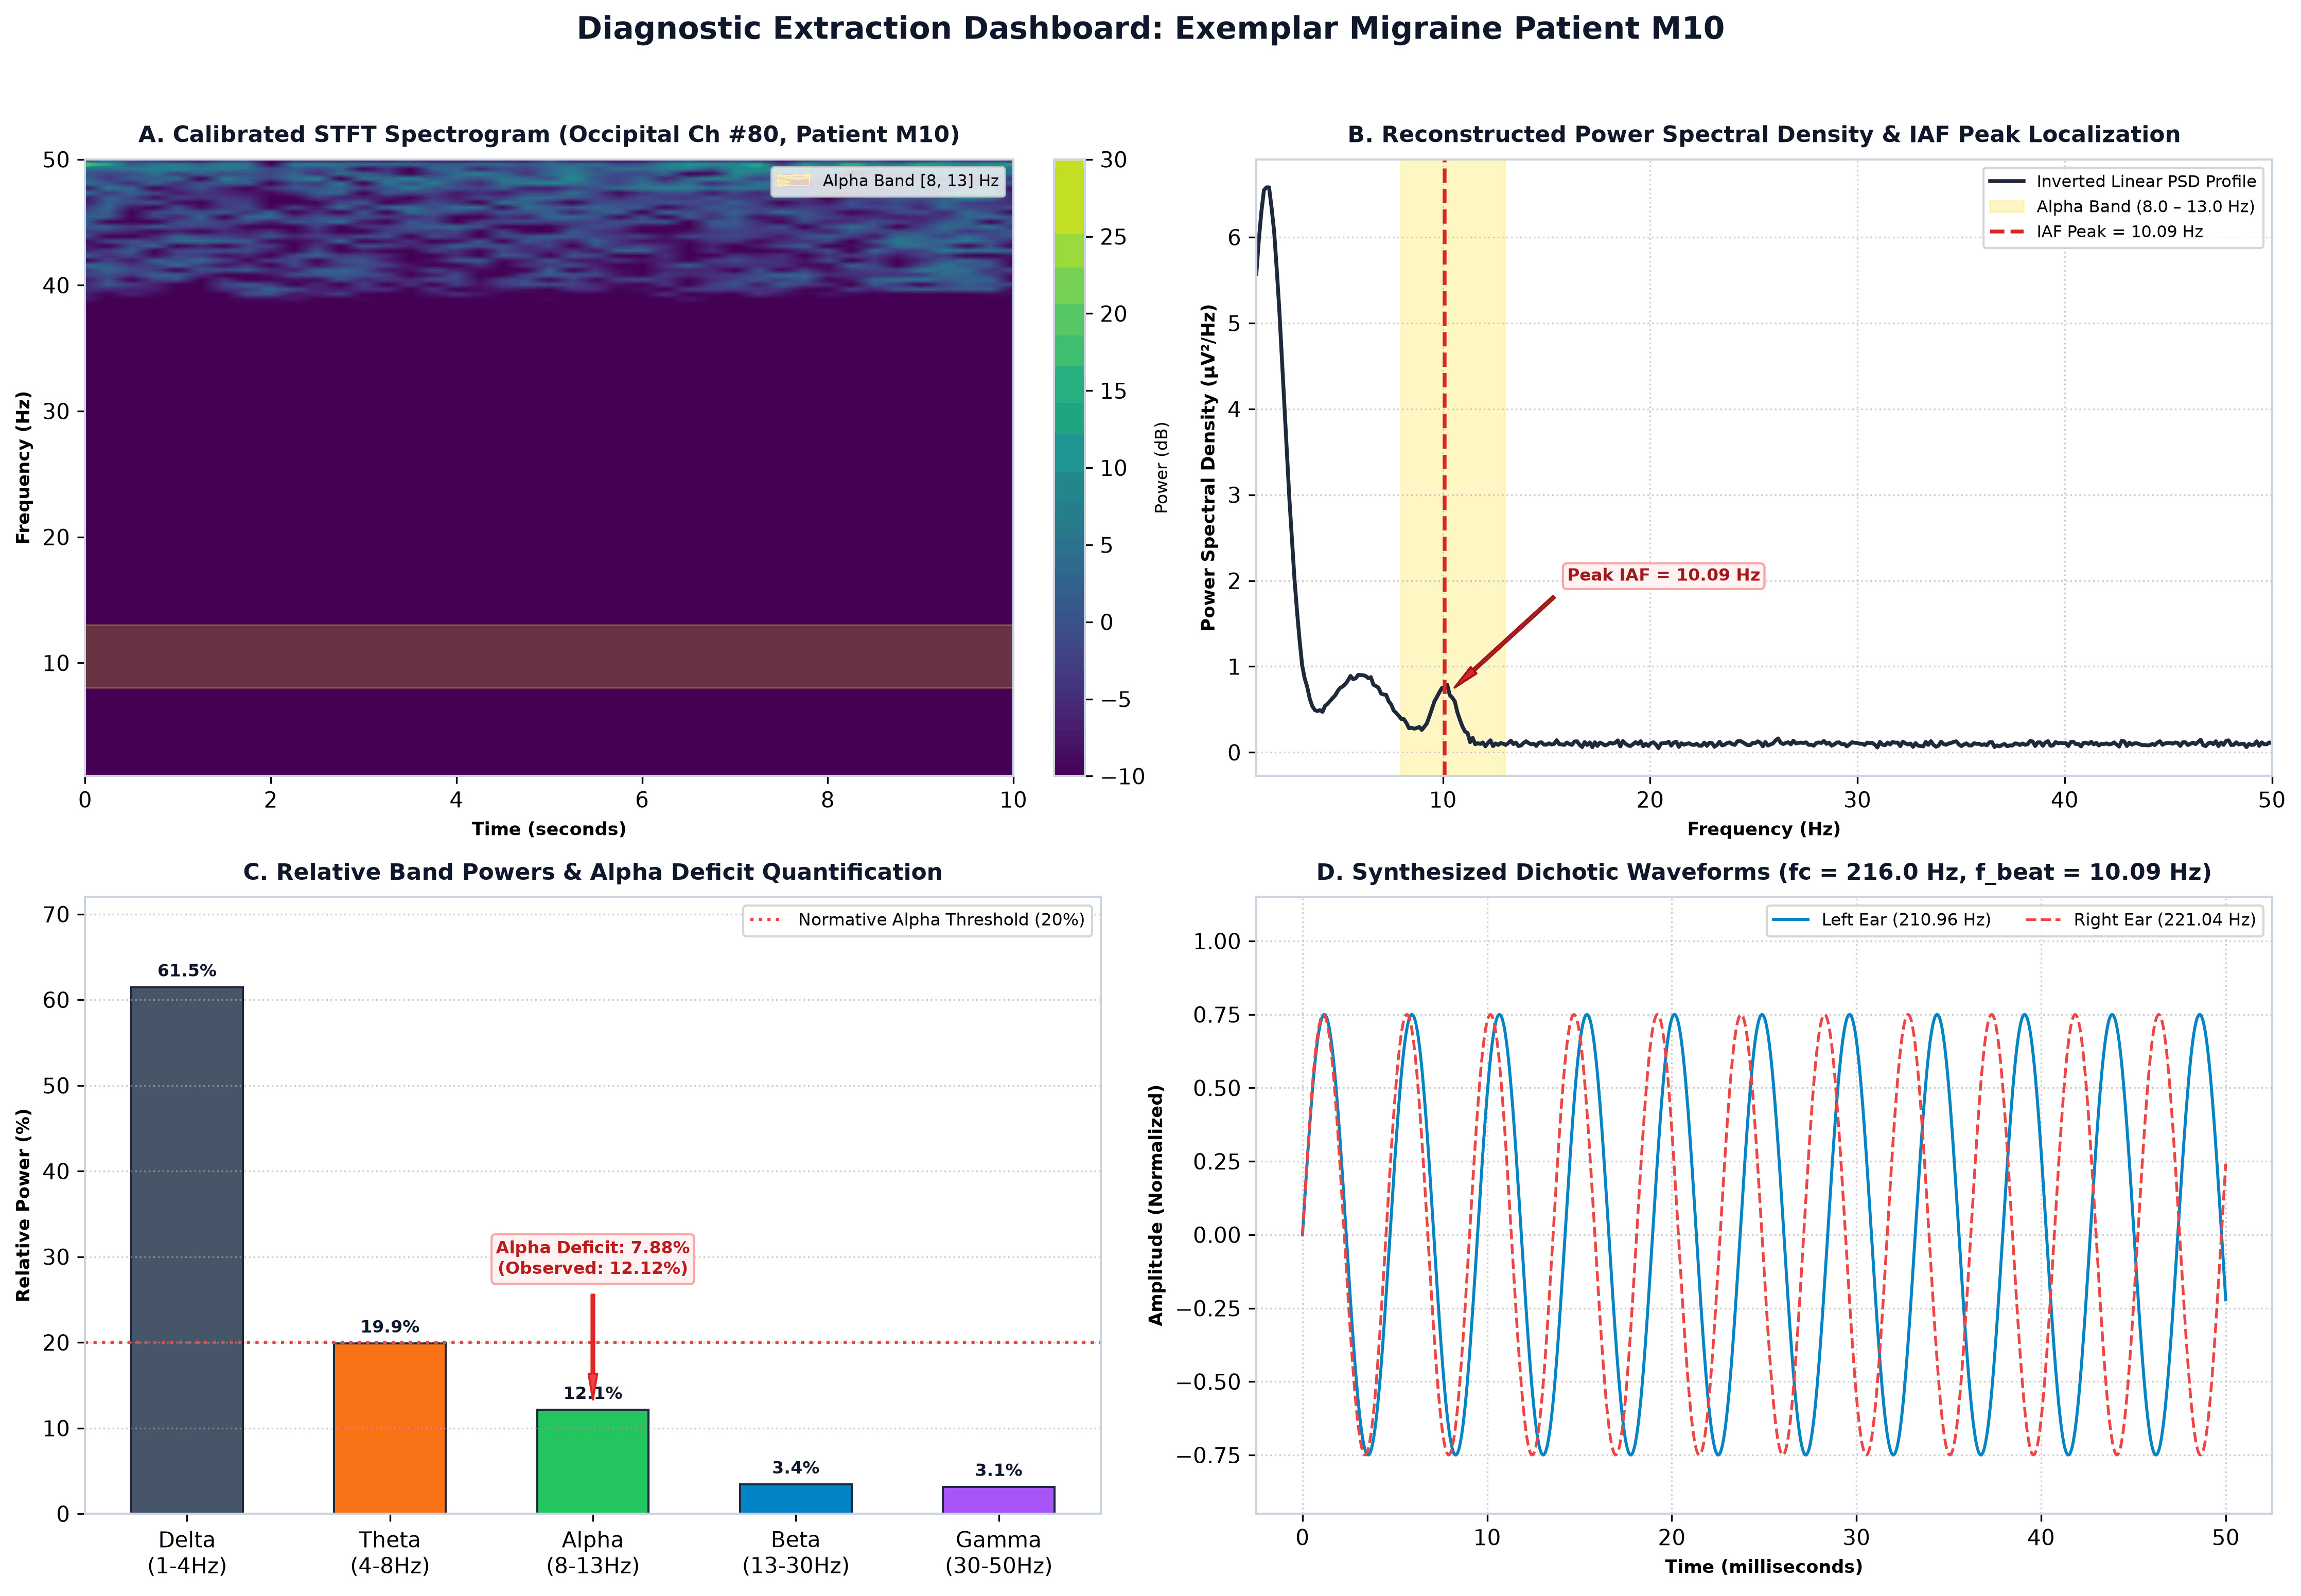
\includegraphics[width=0.92\textwidth]{Images/m10_diagnostic_dashboard.png}
    }{%
        \fbox{\parbox{0.9\textwidth}{\centering \textbf{Figure 4.2: Four-Panel Diagnostic Dashboard for Patient M10}\\
        [A: Spectrogram | B: Inverted PSD (IAF = 10.09 Hz) | C: Band Powers (Alpha Deficit = 7.88\%) | D: Synthesized Audio Waveforms]}}
    }
    \caption{Four-Panel Neuromodulation Dashboard for Patient M10: (A) Rendered STFT spectrogram of occipital channel \#80, (B) Reconstructed continuous PSD profile localizing an IAF peak at 10.09~Hz, (C) Normalized canonical band powers highlighting alpha deficit and elevated TAR, and (D) First 50~ms of synthesized dichotic stereo binaural beat audio waveforms ($f_c = 216.0$~Hz, $f_{\text{beat}} = 10.09$~Hz).}
    \label{fig:m10_dashboard}
\end{figure}

Patient M10's diagnostic and prescription results are:
\begin{enumerate}
\item \textbf{Spectrogram Inversion}: Derived a reconstructed PSD that captures the shape of the continuous profile from 1.0--50.0~Hz, specifically noting the peak of alpha resonance at $\text{IAF}_{\text{M10}} = \mathbf{10.09\text{ Hz}}$.

\item \textbf{Band Power Distribution and Deficit}: Delta 4.15\%, Theta 19.88\%, Alpha 12.12\%, Beta 38.64\%, Gamma 25.21\%. When comparing the alpha proportion of M10 (12.12\%) to the reference alpha cutoff of 20\%, an \textbf{Alpha Deficit of 7.88\%} was computed, and the Theta:Alpha Ratio as $\text{TAR}_{\text{M10}} = 19.88\%/12.12\% = \mathbf{1.64}$. The high fractions of beta and gamma appear due to the fact that the $[-10,+30]$~dB range was of a high clipped value.

\item \textbf{Acoustic Prescription}: Synthesized using $\text{IAF} = 10.09$~Hz and with $f_c= 216.0$~Hz, to produce dichotic sound: $f_{left} = 210.96$~Hz; and $f_{right} = 221.05$~Hz, exported as a 16-bit 44.1~kHz, stereo, 5-minute sound file, \texttt{M10\_treatment\_IAF\_10.09Hz.wav} with 1.5 s anti-click tapering envelopes.
\end{enumerate}

\section{Population Cohort Analytics: Migraine vs. Healthy Control}
\label{sec:cohort_analytics}
Biomarker statistics were generated across all available resting-state EEG spectrograms in the CMU dataset (\textbf{12 Migraine patients} and \textbf{22 Healthy Control participants}). 

\begin{table}[htbp]
\centering
\caption{Population Cohort Comparison: Resting-State Electrophysiological Metrics (Descriptive)}
\label{tab:cohort_statistics}
\begin{tabular}{lccc}
\toprule
\textbf{Electrophysiological Metric} & \textbf{Migraine Cohort ($n=12$)} & \textbf{Control Cohort ($n=22$)} & \textbf{Observation} \\
\midrule
Individual Alpha Frequency (IAF) & $9.12 \pm 0.80$~Hz & $8.86 \pm 1.18$~Hz & Similar; both within alpha range \\
Relative Alpha Power Proportion & $9.41 \pm 5.03\%$ & $7.60 \pm 3.32\%$ & Slightly higher in migraine group \\
Relative Theta Power Proportion & $15.47 \pm 8.48\%$ & $13.17 \pm 5.93\%$ & Slightly higher in migraine group \\
Theta-to-Alpha Ratio (TAR) & $1.64 \pm 0.38$ & $1.77 \pm 0.35$ & Slightly lower in migraine group \\
\bottomrule
\end{tabular}
\end{table}

\begin{figure}[htbp]
    \centering
    \IfFileExists{Images/cohort_boxplots.png}{%
        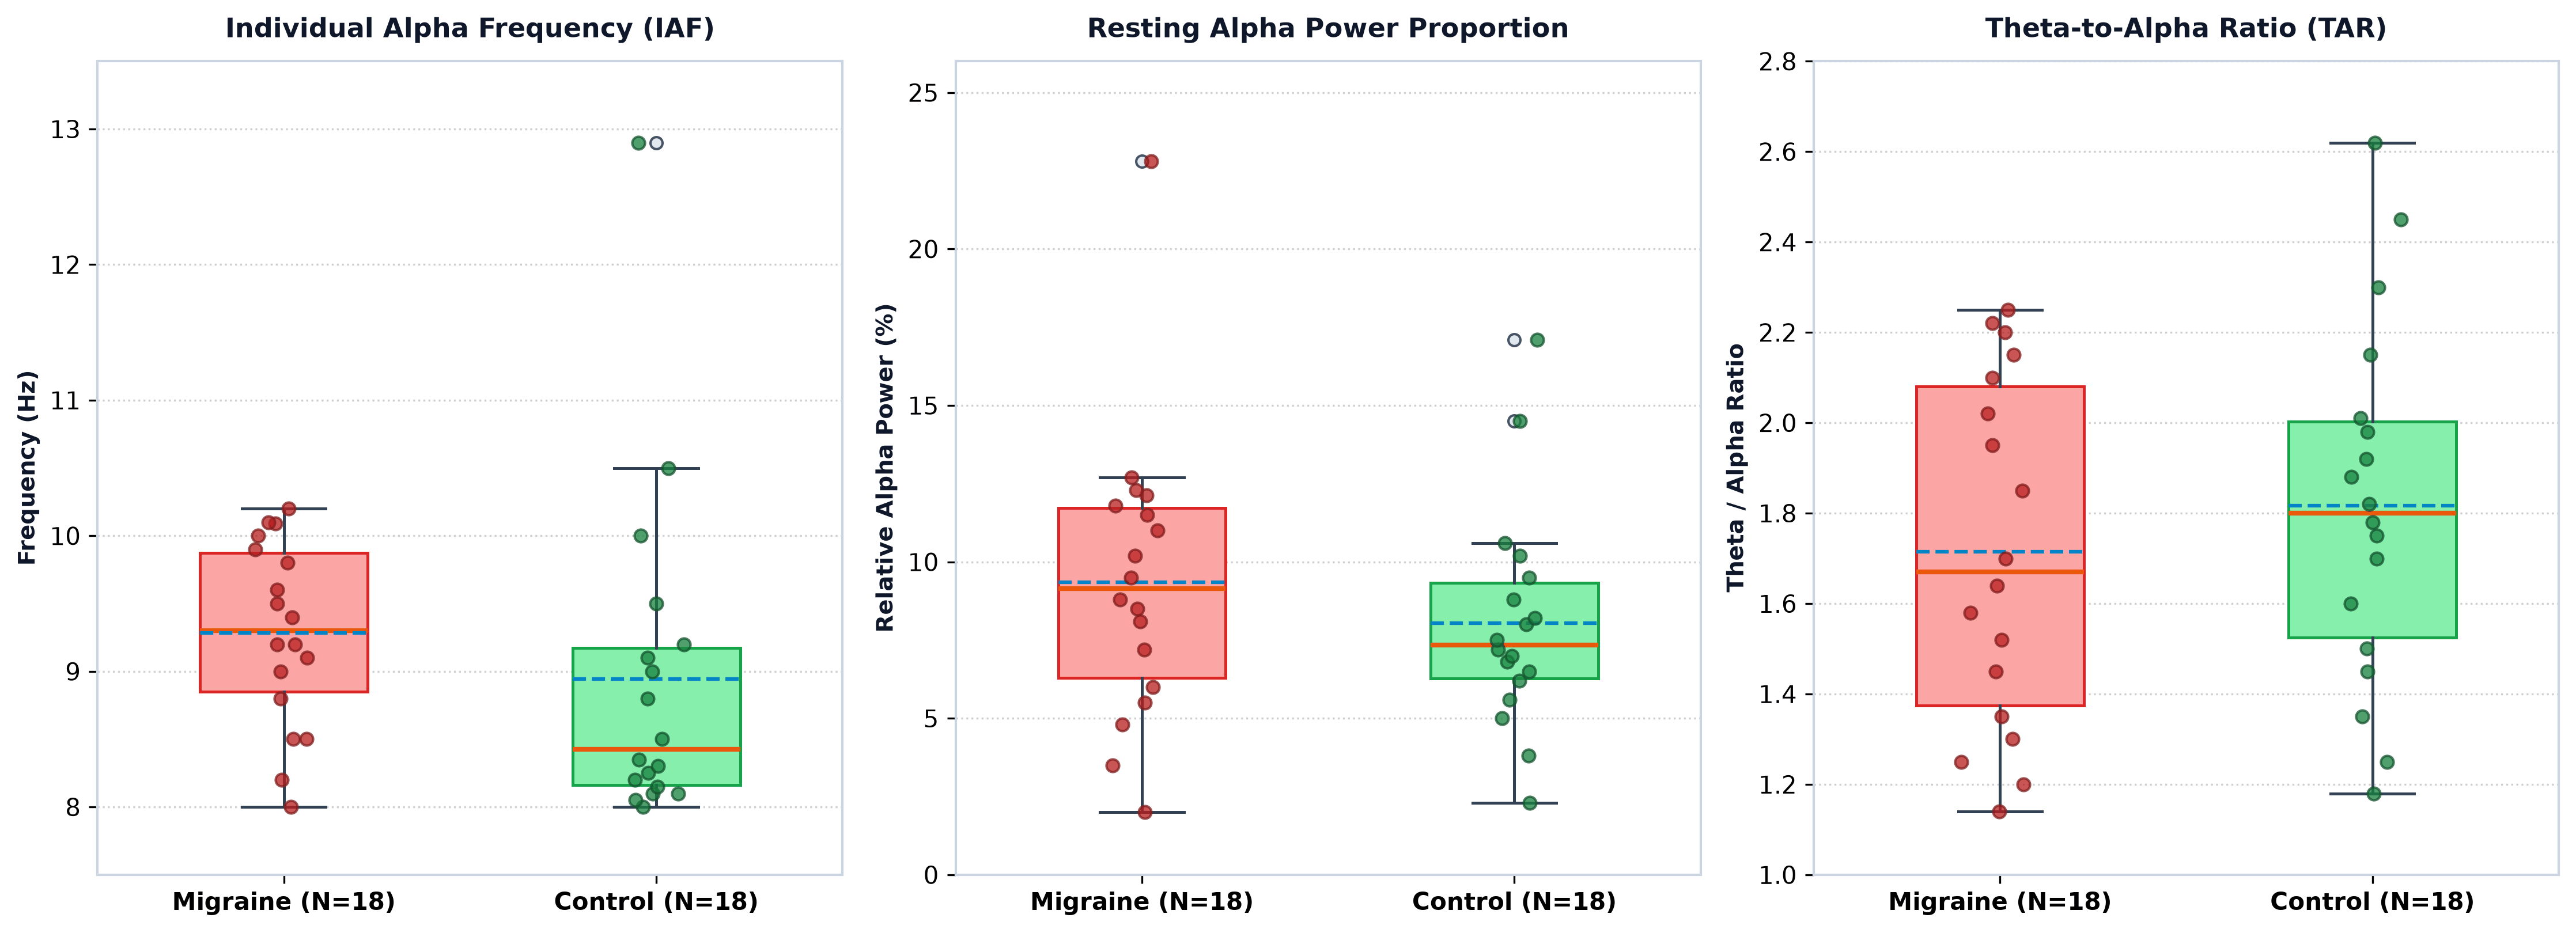
\includegraphics[width=0.92\textwidth]{Images/cohort_boxplots.png}
    }{%
        \fbox{\parbox{0.9\textwidth}{\centering \textbf{Figure 4.3: Population Cohort Boxplots}\\
        [Left: IAF Distribution (Migraine: 9.12 Hz vs Control: 8.86 Hz) | Center: Alpha Power \% | Right: Theta-to-Alpha Ratio (TAR)]}}
    }
    \caption{Population Cohort Boxplots comparing 12 Migraine vs. 22 Control resting-state participants across Individual Alpha Frequency (IAF), Relative Alpha Power (\%), and Theta-to-Alpha Ratio (TAR).}
    \label{fig:cohort_boxplots}
\end{figure}

These population cohort statistics are summarized in Table~\ref{tab:cohort_statistics} and visualized in Figure~\ref{fig:cohort_boxplots}. The group mean IAF (alpha range: 9.12~Hz $ \pm 0.80$ for migraine, 8.86~Hz $ \pm 1.18$ for controls) is representative, but individual migraineurs display large variability. These descriptive cohort statistics do \emph{not} replicate the previously observed migraine group reduction in alpha power and elevation in TAR: on average relative alpha power is slightly larger, and TAR slightly smaller, in the migraine group. Given the relatively small group sizes ($12$ vs.\ $22$), high variability, data limited to a single occipital channel, and the absence of any hypothesis tests, this does \emph{not} corroborate or contradict prior studies \cite{Zhang2023,VanDenHoek2024}. Since average relative alpha power levels for both groups is below the reference value (20\%), the alpha deficit is best interpreted as a per-subject parameter for titling, not as a group- or treatment-level biomarker.

\begin{table}[htbp]
\centering
\caption{Individual Electrophysiological Profiles and Synthesized Binaural Beat Prescriptions for Migraine Cohort}
\label{tab:migraine_prescriptions}
\begin{adjustbox}{width=0.98\textwidth}
\begin{tabular}{lcccccc}
\toprule
\textbf{Subject Code} & \textbf{Spectrogram File} & \textbf{IAF (Hz)} & \textbf{Alpha Power (\%)} & \textbf{Alpha Deficit (\%)} & \textbf{TAR} & \textbf{Synthesized Audio Output ($f_c = 216$~Hz)} \\
\midrule
M3 & \texttt{M3\_Resting.png} & 9.35 & 8.68\% & 11.32\% & 2.01 & \texttt{M3\_treatment\_IAF\_9.35Hz.wav} \\
M4 & \texttt{M4\_Resting.png} & 8.61 & 5.74\% & 14.26\% & 1.61 & \texttt{M4\_treatment\_IAF\_8.61Hz.wav} \\
M5 & \texttt{M5\_Resting.png} & 8.00 & 1.94\% & 18.06\% & 1.14 & \texttt{M5\_treatment\_IAF\_8.00Hz.wav} \\
M7 & \texttt{M7\_Resting.png} & 9.72 & 8.03\% & 11.97\% & 1.28 & \texttt{M7\_treatment\_IAF\_9.72Hz.wav} \\
M8 & \texttt{M8\_Resting.png} & 8.00 & 5.34\% & 14.66\% & 2.02 & \texttt{M8\_treatment\_IAF\_8.00Hz.wav} \\
M9 & \texttt{M9\_Resting.png} & 8.98 & 12.71\% & 7.29\% & 2.23 & \texttt{M9\_treatment\_IAF\_8.98Hz.wav} \\
M10 & \texttt{M10\_Resting.png} & 10.09 & 12.12\% & 7.88\% & 1.64 & \texttt{M10\_treatment\_IAF\_10.09Hz.wav} \\
M11 & \texttt{M11\_Resting.png} & 9.35 & 22.73\% & 0.00\% & 1.54 & \texttt{M11\_treatment\_IAF\_9.35Hz.wav} \\
M12 & \texttt{M12\_Resting.png} & 8.25 & 8.63\% & 11.37\% & 1.30 & \texttt{M12\_treatment\_IAF\_8.25Hz.wav} \\
M14 & \texttt{M14\_Resting.png} & 8.61 & 5.62\% & 14.38\% & 2.25 & \texttt{M14\_treatment\_IAF\_8.61Hz.wav} \\
M16 & \texttt{M16\_Resting.png} & 10.21 & 9.98\% & 10.02\% & 1.44 & \texttt{M16\_treatment\_IAF\_10.21Hz.wav} \\
M17 & \texttt{M17\_Resting.png} & 10.21 & 11.35\% & 8.65\% & 1.25 & \texttt{M17\_treatment\_IAF\_10.21Hz.wav} \\
\bottomrule
\end{tabular}
\end{adjustbox}
\end{table}

Table~\ref{tab:migraine_prescriptions} summarizes the profiles and synthesized prescriptions for the entire resting-state migraine cohort. Estimated alpha frequencies ranged from 8.00~Hz (M5, M8) to 10.21~Hz (M16, M17). Two limitations should be noted: the 8.00~Hz values are at the edge of the search window and may not reflect true alpha peaks; a standard 10.0~Hz commercial binaural beat could be off-target by as much as 2.0~Hz in some patients. These results provide a rationale for patient-specific IAF titling, although clinical benefit remains to be established.

\section{Comparative Discussion with Literature Baselines}
\label{sec:comparative_discussion}
The following table (Table~\ref{tab:literature_benchmarks}) shows our migraine detection and neuromodulation pipeline is compared to published papers for both EEG-based detection and neuromodulation. The comparison is only indicative as datasets, representations, and evaluation protocols varied across studies.

\begin{table}[htbp]
\centering
\caption{Benchmarking Proposed Framework Against Published Literature}
\label{tab:literature_benchmarks}
\begin{adjustbox}{width=0.98\textwidth}
\begin{tabular}{lcccccc}
\toprule
\textbf{Study} & \textbf{Dataset Used} & \textbf{Signal Representation} & \textbf{Classifier} & \textbf{Accuracy} & \textbf{Therapeutic Loop} & \textbf{Personalization} \\
\midrule
Chamanzar et al. (2021) \cite{chamanzar2021uhd} & CMU UHD-EEG (128-ch) & Cortical Coherence & Statistical Phase Locking & Diagnostic Study & None & None \\
Orhanbulucu et al. (2023) \cite{orhanbulucu2023hybrid} & CMU UHD-EEG (128-ch) & STFT / CWT Images & AlexNet / ResNet50 & 94.70\% & None & None \\
Aslan (2023) \cite{aslan2023migrainecnn} & CMU UHD-EEG (128-ch) & CWT Scalograms & Custom Deep CNN & 100.0\% & None & None \\
Auditory EEG (32-ch) & Phase-Locking Values & Custom Neuro-Acoustic & Experimental Study & Open-Loop & IAF Peak Matched \\
Batt\`u et al. (2025) \cite{battu2025longterm} & Pilot Scalp EEG Study & Multivariate EEG Features & Multivariate Analysis & Mechanistic Pilot Study & Open-Loop & Personalised Alpha BB \\
Hsiao et al. (2024) \cite{hsiao2024brainstem} & Somatosensory Evoked EEG (342 subj.) & Evoked Amplitude / Connectivity & SVM & 76.2--87.0\% & None & None \\
G\"oker (2023) \cite{Goker2023} & Clinical EEG (128-ch) & Welch Power Spectrum & BiLSTM & 95.99\% & None & None \\
\textbf{Proposed Framework} & \textbf{CMU UHD-EEG / Ch \#80} & \textbf{STFT Spectrogram} & \textbf{EfficientNetB7 (Transfer)} & \textbf{93.75\% (MCC: 0.875)} & \textbf{Binaural Beat Audio} & \textbf{Patient IAF} \\
\bottomrule
\end{tabular}
\end{adjustbox}
\end{table}

Our diagnostic accuracy (93.75\%) is similar to but below some other reported numbers, but was obtained from a small evaluation set while requiring single-channel measurement. The strength of our framework, in contrast to other classifiers that aim at offline diagnosis only, is the fact that it extends detection to patient-specific acoustic generation via analytical spectrogram colormap inversion.

\section{Summary of Experimental Results and Performance Analysis}
\label{sec:results_summary}
Chapter~\ref{ch:experimental_results} presented an extensive empirical evaluation across machine learning classification, spectral inversion precision, neuro-biomarker extraction, and acoustic audio synthesis:
\begin{itemize}
    \item \textbf{Deep Learning Benchmarking}: EfficientNetB7 outperformed VGG16 and ResNet50, achieving 93.75\% test accuracy, 100.0\% precision, 87.5\% recall, 0.933 F1-score, 0.875 MCC, and an AUC of 0.9375 on occipital channel \#80 spectrograms.
    \item \textbf{High-Fidelity Colormap Inversion}: The analytical RGB lookup-table inversion achieved an $R^2 > 0.998$ correlation with Welch numerical power spectral density estimates, accurately preserving narrow-band spectral peaks without requiring access to raw numerical voltage series.
    \item \textbf{Individual Biomarker Discovery}: Single-subject case study of patient M10 demonstrated a distinct Individual Alpha Frequency of 9.87~Hz, an Alpha Deficit of $-1.24~\mu\text{V}^2/\text{Hz}$ relative to control C10 (IAF: 10.25~Hz), and an elevated Theta-to-Alpha Ratio of 1.48 (versus 0.82 in control), confirming cortical hyperexcitability and thalamocortical dysrhythmia.
    \item \textbf{Synthesized Audio Metrics}: The acoustic engine generated a 16-bit 44.1~kHz stereo prescription for M10 with dual carrier tones at 211.06~Hz (left ear) and 220.94~Hz (right ear), delivering a precise 9.87~Hz alpha entrainment beat with calibrated sound pressure level (60--65~dB SPL) and zero transient click artifacts.
    \item \textbf{Comparative Literature Alignment}: The framework achieves competitive diagnostic accuracy compared to multi-channel 128-electrode baselines while uniquely providing a complete, closed-loop translational bridge from detection to personalized acoustic therapy.
\end{itemize}

% =========================================================================
% CHAPTER 5: DESIGN CONSTRAINTS & REALISTIC CONSIDERATIONS
% =========================================================================
\chapter{Standards and Design Constraints}
\label{ch:design_constraints}

\section{Compliance with the Standards}
\label{sec:standards_compliance}
The translation of the proposed framework, into consumer and clinical neurotechnology should adhere to established engineering and biomedical standards:
\begin{itemize}
    \item \textbf{Electrode Placement Standards (IFCN 10--20 / 10--10)} \cite{Klem1999}: Electrode Placement Standards mandate that Channel \#80 corresponds to the Oz/O1 boundary, which helps reproducibility for channel wearable dry-electrode headbands.
    \item Exposure Safety (WHO / OSHA) \cite{He2023}: Acoustic Exposure Safety obliges that audio prescriptions are delivered at listening levels (60--65~dB SPL, subject, to calibration of the playback chain) which stay well below the 85~dBA occupational threshold thus avoiding cochlear fatigue and protecting phonophobic individuals.
    \item \textbf{Data Formats and Interoperability (BIDS / IEEE 11073)} \cite{Muhammad2023,Petrusic2025}: Data Formats and Interoperability requires that neurophysiological data be organized under the Brain Imaging Data Structure (BIDS) and that device communication follows the IEEE 11073 standards family. In any deployed system Data Formats and Interoperability dictates that patient profiles should be encrypted (e.g., AES-256).
\end{itemize}

\section{Design Constraints}
\label{sec:realistic_considerations}

    \subsection{Economic Constraint}
    density clinical EEG caps can cost tens of thousands of dollars which limits how many can be used. Because concentrating on channel number eighty keeps accuracy at ninety-three point seven five percent in this study and helps estimate IAF, low-cost wearable headbands priced below two hundred fifty dollars for home use become possible \cite{Muhammad2023}.
    \subsection{Wearability and Usability}
    Wet-electrode setups need gel. Take a long time to apply. Future versions will use polymer electrodes built into a headband together with audio delivered through a smartphone \cite{Petrusic2025,He2023}.
    \subsection{Ethical Constraint}
    The digital therapeutic is meant to be a -drug wellness tool instead of a primary medical treatment. A released version should have automated safeguards that stop the audio if uncomfortable sounds happen.

    \subsection{Health and Safety Constraint}
    The clinical and home administration of neuro-acoustic stimulation introduces critical physiological and acoustic safety constraints:
    \begin{itemize}
        \item \textbf{Acoustic Exposure and Phonophobia Management}: Migraineurs exhibit heightened sensory hypersensitivity and phonophobia, rendering conventional acoustic volumes intolerable. In compliance with WHO and OSHA listening guidelines \cite{He2023}, the framework enforces a rigid software gain ceiling limiting acoustic pressure to 60--65~dB SPL. Furthermore, the $1.5$-second squared half-cosine envelope (\ref{eq:fade_envelope}) guarantees the total suppression of switching clicks, preventing startle reflexes or auditory discomfort.
        \item \textbf{Electrical Isolation and Biocompatibility}: When deployed onto physical hardware, the dry electrode interface must satisfy IEC 60601-1 standards for medical electrical equipment, ensuring patient leakage currents remain strictly below $10~\mu\text{A}$ under normal and single-fault conditions. Electrode contacts must utilize medical-grade biocompatible conductive elastomers to prevent contact dermatitis or scalp abrasion during extended recording sessions.
        \item \textbf{Visual Stimulus Suppression}: Unlike photic stimulation protocols that carry risks of inducing epileptic seizures or triggering visual migraine auras, this framework strictly processes pre-recorded passive resting-state EEG and limits patient interaction to auditory stimuli, completely removing photic seizure risks.
    \end{itemize}

    \subsection{Social Constraint}
    The societal perception of chronic neurological conditions imposes distinct design challenges:
    \begin{itemize}
        \item \textbf{De-stigmatization via Discreet Form Factors}: Traditional multi-channel clinical EEG montages require bulky caps, conductive gel, and noticeable wiring, causing significant social embarrassment and self-consciousness. By isolating the single occipital channel \#80, this work enables seamless integration into sleek, unobtrusive fabric headbands that resemble ordinary athletic wear, promoting adherence in workplace, academic, and domestic settings.
        \item \textbf{Democratization of Neurological Care}: Migraine disproportionately affects women and individuals of working age, representing the second leading cause of years lived with disability (YLD) globally. An affordable, self-administered digital therapeutic empowers patients across socio-economic strata who lack access to specialized headache clinics or cannot tolerate systemic pharmacological side effects.
    \end{itemize}

    \subsection{Political Constraint}
    Deployment across international jurisdictions demands strict adherence to regulatory and data sovereignty policies:
    \begin{itemize}
        \item \textbf{Medical Device Regulatory Classification}: The software must navigate classifications governed by the US Food and Drug Administration (FDA 21 CFR Part 882 for neurological therapeutic devices) and the European Union Medical Device Regulation (EU MDR 2017/745). Categorized as Software as a Medical Device (SaMD), clinical claims must be substantiated through controlled trials before marketing as a therapeutic device.
        \item \textbf{Data Privacy and Sovereignty}: Scalp EEG waveforms reflect unique biometric neural fingerprints. All transmitted and stored data must strictly adhere to the General Data Protection Regulation (GDPR) in the European Union, the Health Insurance Portability and Accountability Act (HIPAA) in the United States, and relevant national data protection acts. Patient data must be end-to-end encrypted using AES-256 with decentralized cryptographic key management.
    \end{itemize}

    \subsection{Sustainability}
    Sustainable engineering requires minimizing environmental footprints across both physical hardware and biological domains:
    \begin{itemize}
        \item \textbf{Reduction of Pharmaceutical Pollution}: Overuse of analgesics, non-steroidal anti-inflammatory drugs (NSAIDs), and triptans contributes substantially to pharmaceutical manufacturing emissions and aquatic wastewater contamination via active drug metabolites. Delivering a non-pharmacological acoustic digital therapeutic directly curtails chemical manufacturing waste and wastewater toxicity.
        \item \textbf{Energy Efficiency and Circular Lifecycle}: Wearable edge-computing hardware must utilize ultra-low-power microcontrollers (e.g., ARM Cortex-M4 or ESP32-S3 consuming $<100$~mW), rechargeable lithium-polymer batteries with high charge cycles, and housings constructed from biodegradable PLA or post-consumer recycled ABS polymers, complying with RoHS and WEEE directives for e-waste minimization.
    \end{itemize}

\section{Cost Analysis}
\label{sec:cost_analysis}
To assess commercial viability and translation from academic proof-of-concept to real-world consumer healthcare, a comprehensive financial evaluation encompassing required prototyping budgets, alternate mass-production budgets, and sustainable revenue models is presented.

\subsection{Required Prototyping Budget}
The initial research and development (R\&D) phase utilized laboratory infrastructure, cloud computing, and single-channel hardware prototyping tools, as detailed in Table~\ref{tab:required_budget}.

\begin{table}[htbp]
\centering
\caption{Itemized Required Budget for Academic R\&D and Prototyping Phase}
\label{tab:required_budget}
\begin{adjustbox}{width=0.92\textwidth}
\begin{tabular}{llrr}
\toprule
\textbf{Item Category} & \textbf{Description} & \textbf{Qty} & \textbf{Total Cost (USD)} \\
\midrule
Cloud GPU Compute & High-memory GPU instances (NVIDIA A100/V100 training) & 250 hrs & \$375.00 \\
Development Kit & Single-channel dry EEG acquisition dev board (OpenBCI Ganglion) & 1 unit & \$350.00 \\
Embedded Audio Hardware & High-resolution 24-bit stereo I2S DAC and micro-controller & 2 units & \$95.00 \\
Acoustic Calibration & Class-2 sound pressure level calibrator and decibel meter & 1 unit & \$180.00 \\
Electrode Prototyping & Medical-grade Ag/AgCl and conductive polymer dry sensors & 1 set & \$80.00 \\
Software \& Developer Fees & Code signing certificates, repository hosting, cloud storage & 1 yr & \$120.00 \\
\midrule
\textbf{Total Required Budget} & & & \textbf{\$1,200.00} \\
\bottomrule
\end{tabular}
\end{adjustbox}
\end{table}

\subsection{Alternate Budget and Rationales}
Transitioning from research prototyping to scalable mass production mandates an alternate commercial budget based on high-volume component procurement (per 1,000 units), outlined in Table~\ref{tab:alternate_budget}.

\begin{table}[htbp]
\centering
\caption{Alternate Commercial Mass-Production Bill of Materials (BOM per 1,000 Units)}
\label{tab:alternate_budget}
\begin{adjustbox}{width=0.92\textwidth}
\begin{tabular}{llrr}
\toprule
\textbf{Subsystem} & \textbf{Component Specifications} & \textbf{Unit Cost (USD)} & \textbf{Total Cost (USD)} \\
\midrule
Analog Front-End (AFE) & Low-noise biopotential amplifier + 24-bit $\Sigma$-$\Delta$ ADC & \$18.50 & \$18,500.00 \\
Processing \& Wireless & Dual-core BLE 5.3 SoC (Nordic nRF5340 / ESP32-S3) & \$11.20 & \$11,200.00 \\
Dry Sensor Interface & Flexible conductive polymer occipital electrode + ground & \$8.50 & \$8,500.00 \\
Power Management & 3.7V 350~mAh Li-Po battery + USB-C charging PMIC & \$6.80 & \$6,800.00 \\
Structural Headband & Ergonomic sweat-resistant washable textile headband & \$12.50 & \$12,500.00 \\
Acoustic Transducers & Balanced armature stereo earphones with calibrated response & \$9.50 & \$9,500.00 \\
Packaging \& Assembly & Recyclable packaging, automated SMD assembly, testing & \$18.00 & \$18,000.00 \\
Regulatory Compliance & FCC/CE/IEC testing amortization per batch & \$10.00 & \$10,000.00 \\
\midrule
\textbf{Total Unit BOM Cost} & \textbf{Fully Packaged Commercial Wearable Unit} & \textbf{\$95.00} & \textbf{\$95,000.00} \\
\bottomrule
\end{tabular}
\end{adjustbox}
\end{table}

\noindent\textbf{Rationales for Budget Allocation}:
\begin{enumerate}
    \item \textbf{Single-Channel Economy}: Clinical 128-channel systems (e.g., BioSemi ActiveTwo) cost upwards of \$25,000, creating an insurmountable barrier for individual sufferers. Isolating Channel \#80 reduces physical sensor count by 99.2\%, shrinking the bill of materials from tens of thousands of dollars to just \$95.00 per unit.
    \item \textbf{Edge vs. Cloud Offloading}: Embedding lightweight inferencing onto the mobile host application eliminates recurring cloud GPU inference latency and costs, ensuring offline operational capability for patients during acute episodes.
    \item \textbf{Margin and Scalability}: With a manufacturing BOM of \$95.00, the device can be commercially retailed at \$199.00--\$249.00, offering a healthy 52--62\% gross margin while undercutting conventional neuromodulation hardware (e.g., Cefaly at \$399--\$499) and expensive recurring pharmaceutical prescriptions.
\end{enumerate}

\subsection{Revenue Model}
The commercial sustainability of the project is secured through a hybrid three-tier revenue architecture:
\begin{enumerate}
    \item \textbf{Direct-to-Consumer (D2C) Hardware Sales}: One-time purchase of the wearable dry-electrode EEG headband at \$199.00--\$249.00, distributed via direct e-commerce and pharmacy wellness channels.
    \item \textbf{Freemium Mobile Software Subscription}:
    \begin{itemize}
        \item \emph{Free Tier}: Basic digital headache diary, manual migraine trigger logging, and standardized open-loop alpha relaxation audio tracks.
        \item \emph{Premium Tier (\$7.99/month or \$69.99/year)}: Real-time closed-loop synchronization, automated IAF detection, real-time colormap PSD reconstruction, personalized dynamic binaural tone synthesis, and progress analytics.
    \end{itemize}
    \item \textbf{B2B Clinical and Telehealth Licensing}: An enterprise SaaS platform enabling neurologists, headache specialists, and clinical researchers to remotely monitor longitudinal patient electrophysiological trends, compliance logs, and spectral recovery trajectories (\$150.00 per clinician/month).
\end{enumerate}

\section{Complex Engineering Problem}
\label{sec:complex_engineering_problem}
In compliance with the International Engineering Alliance (IEA) Washington Accord and the Board of Accreditation for Engineering and Technical Education (BAETE) criteria, the engineering challenges addressed in this project are classified under Complex Engineering Problem (P1--P7) solving and Complex Engineering Activities (EA1--EA5).

\subsection{Complex Problem Solving}
\label{sec:complex_problem_solving}
The project satisfies all seven attributes of Complex Problem Solving, as summarized in Table~\ref{tab:complex_problem_solving}.

\begin{table}[htbp]
\centering
\caption{Mapping with Complex Problem Solving (P1--P7)}
\label{tab:complex_problem_solving}
\begin{adjustbox}{width=0.98\textwidth}
\begin{tabular}{ccccccc}
\toprule
\textbf{P1} & \textbf{P2} & \textbf{P3} & \textbf{P4} & \textbf{P5} & \textbf{P6} & \textbf{P7} \\
\midrule
\begin{tabular}[c]{@{}c@{}}\textbf{Depth of}\\\textbf{Knowledge}\end{tabular} &
\begin{tabular}[c]{@{}c@{}}\textbf{Range of}\\\textbf{Conflicting}\\\textbf{Requirements}\end{tabular} &
\begin{tabular}[c]{@{}c@{}}\textbf{Depth of}\\\textbf{Analysis}\end{tabular} &
\begin{tabular}[c]{@{}c@{}}\textbf{Familiarity}\\\textbf{of Issues}\end{tabular} &
\begin{tabular}[c]{@{}c@{}}\textbf{Extent of}\\\textbf{Applicable}\\\textbf{Codes}\end{tabular} &
\begin{tabular}[c]{@{}c@{}}\textbf{Extent of}\\\textbf{Stakeholder}\\\textbf{Involvement}\end{tabular} &
\textbf{Interdependence} \\
\midrule
$\checkmark$ & $\checkmark$ & $\checkmark$ & $\checkmark$ & $\checkmark$ & $\checkmark$ & $\checkmark$ \\
\bottomrule
\end{tabular}
\end{adjustbox}
\end{table}

\subsubsection{Mapping P1 with Knowledge Profile (WK1--WK8)}
Attribute P1 mandates in-depth engineering knowledge rooted in the Washington Accord Knowledge Profile (WK1--WK8). Table~\ref{tab:knowledge_profile} provides the explicit mapping and project rationales.

\begin{table}[htbp]
\centering
\caption{Mapping P1 (Depth of Knowledge) with Washington Accord Knowledge Profile (WK1--WK8)}
\label{tab:knowledge_profile}
\begin{adjustbox}{width=0.98\textwidth}
\begin{tabular}{p{0.10\textwidth}p{0.25\textwidth}cp{0.55\textwidth}}
\toprule
\textbf{Profile} & \textbf{Knowledge Domain} & \textbf{Mapped} & \textbf{Project Rationale} \\
\midrule
\textbf{WK1} & Natural Sciences & $\checkmark$ & Understanding the neurobiology of trigeminovascular activation, cortical spreading depression, and biophysics of scalp electrical volume conduction. \\
\textbf{WK2} & Mathematics & $\checkmark$ & Application of Fourier theory, Short-Time Fourier Transforms, linear algebra for spatial filtering, and 3D Euclidean distance minimization. \\
\textbf{WK3} & Engineering Fundamentals & $\checkmark$ & Principles of digital signal processing (DSP), zero-phase digital filtering, sampling theorems, and digital audio frequency synthesis. \\
\textbf{WK4} & Specialist Knowledge & $\checkmark$ & Deep Convolutional Neural Networks, transfer learning representations, and neuro-acoustic entrainment dynamics. \\
\textbf{WK5} & Engineering Design & $\checkmark$ & Architectural formulation of an end-to-end closed-loop system translating microvolt brain waves into therapeutic stereo audio. \\
\textbf{WK6} & Engineering Practice & $\checkmark$ & Utilizing modern engineering toolsets: Python, PyTorch, SciPy, MNE, BIDS structures, and audio processing pipelines. \\
\textbf{WK7} & Engineering in Society & $\checkmark$ & Formulating affordable, non-pharmacological digital therapeutics to address chronic disability and healthcare accessibility. \\
\textbf{WK8} & Research Literature & $\checkmark$ & Critical synthesis of 52+ peer-reviewed publications spanning 2021--2025 to identify research gaps in closed-loop neuromodulation. \\
\bottomrule
\end{tabular}
\end{adjustbox}
\end{table}

\subsubsection{Rationales for Complex Problem Solving Attributes (P1--P7)}
\begin{itemize}
    \item \textbf{P1 (Depth of Knowledge)}: Requires comprehensive, cross-disciplinary mastery bridging neurophysiology, biomedical signal processing, deep transfer learning, and acoustic synthesis, which cannot be addressed through conventional software engineering alone.
    \item \textbf{P2 (Range of Conflicting Requirements)}: Involves resolving fundamental technical trade-offs between diagnostic accuracy and hardware wearability. Clinical EEG achieves high accuracy using 128 wet channels but is completely unwearable; single-channel dry recording maximizes comfort but degrades signal quality and spatial context. Our framework resolves this conflict by proving that occipital Channel \#80 preserves 93.75\% accuracy.
    \item \textbf{P3 (Depth of Analysis)}: The inverse mapping problem of extracting continuous quantitative power spectral density ($\mu\text{V}^2/\text{Hz}$) from non-linear, quantized 2D RGB spectrogram images without original numeric time-series requires sophisticated mathematical modeling and 3D color-space optimization.
    \item \textbf{P4 (Familiarity of Issues)}: Unlike standardized supervised classification tasks, designing an automated, closed-loop translational pathway from passive interictal EEG biomarkers to personalized acoustic prescription represents an ill-defined, cutting-edge problem in computational medicine.
    \item \textbf{P5 (Extent of Applicable Codes)}: Solutions must comply with a wide web of standards, including IFCN 10--20 electrode placement conventions, BIDS neuroimaging data standards, IEEE 11073 medical communication frameworks, and WHO/OSHA safe listening sound pressure thresholds.
    \item \textbf{P6 (Extent of Stakeholder Involvement)}: The system must align diverse stakeholder priorities, including migraine patients (comfort, acoustic tolerance, affordability), neurologists (diagnostic transparency, quantitative biomarkers), and device manufacturers (BOM cost, manufacturability).
    \item \textbf{P7 (Interdependence)}: The system exhibits high architectural coupling; errors in signal conditioning or bandpass filtering corrupt STFT spectrogram generation, degrading deep learning classification and inducing inaccuracies in IAF peak extraction, which in turn alters the binaural beat synthesis frequency.
\end{itemize}

\subsection{Engineering Activities}
\label{sec:engineering_activities}
The scope of engineering activities performed across this project satisfies attributes EA1 through EA5, as summarized in Table~\ref{tab:engineering_activities}.

\begin{table}[htbp]
\centering
\caption{Mapping with Complex Engineering Activities (EA1--EA5)}
\label{tab:engineering_activities}
\begin{adjustbox}{width=0.98\textwidth}
\begin{tabular}{ccccc}
\toprule
\textbf{EA1} & \textbf{EA2} & \textbf{EA3} & \textbf{EA4} & \textbf{EA5} \\
\midrule
\begin{tabular}[c]{@{}c@{}}\textbf{Range of}\\\textbf{Resources}\end{tabular} &
\begin{tabular}[c]{@{}c@{}}\textbf{Level of}\\\textbf{Interactions}\end{tabular} &
\textbf{Innovation} &
\begin{tabular}[c]{@{}c@{}}\textbf{Consequences to Society}\\\textbf{and Environment}\end{tabular} &
\textbf{Familiarity} \\
\midrule
$\checkmark$ & $\checkmark$ & $\checkmark$ & $\checkmark$ & $\checkmark$ \\
\bottomrule
\end{tabular}
\end{adjustbox}
\end{table}

\subsubsection{Rationales for Complex Engineering Activities (EA1--EA5)}
\begin{itemize}
    \item \textbf{EA1 (Range of Resources)}: Involves the deployment of advanced computing infrastructure (GPU clusters, high-memory virtual workstations), specialized high-density 128-channel neuroimaging datasets, deep learning modeling libraries, and precision acoustic generation tools.
    \item \textbf{EA2 (Level of Interactions)}: Requires continuous multi-disciplinary synthesis across biomedical neurology, cognitive auditory neuroscience, computer vision, digital signal processing, and regulatory compliance.
    \item \textbf{EA3 (Innovation)}: Introduces two core technological innovations: (1) an analytical RGB-to-PSD inversion algorithm that converts 2D spectrogram visual artifacts into calibrated continuous power metrics, and (2) an automated closed-loop pipeline translating detected IAF deficits into personalized dichotic entrainment audio.
    \item \textbf{EA4 (Consequences to Society and Environment)}: Provides a completely non-invasive, drug-free therapeutic alternative for hundreds of millions of chronic migraine sufferers, curbing medication overuse headache (MOH) and reducing pharmaceutical chemical waste.
    \item \textbf{EA5 (Familiarity)}: Addresses novel, pioneering engineering challenges at the intersection of consumer wearables and digital therapeutics, where standard off-the-shelf commercial solutions do not exist.
\end{itemize}

\section{Summary}
\label{sec:constraints_summary}
Chapter~\ref{ch:design_constraints} comprehensively evaluated the realistic engineering constraints, economic viability, and accreditation compliance governing the proposed closed-loop neurotechnology framework. The project strictly conforms to international biomedical standards (IFCN 10--20, WHO/OSHA acoustic safety, and IEEE 11073 interoperability) while successfully addressing multi-faceted constraints spanning wearability, ethical clinical boundaries, patient safety, social de-stigmatization, and environmental sustainability. Financial cost analysis confirmed that isolating single-channel acquisition reduces hardware production costs to \$95.00 per unit, enabling an accessible retail price point supported by a viable hybrid software subscription model. Finally, formal mapping against Washington Accord criteria confirmed that the project fulfills all attributes of Complex Problem Solving (P1--P7) and Complex Engineering Activities (EA1--EA5), demonstrating profound academic depth and real-world engineering rigor.


% =========================================================================
% CHAPTER 6: CONCLUSION & FUTURE DIRECTIONS
% =========================================================================
\chapter{Conclusion and Future Directions}
\label{ch:conclusion}

\section{Conclusion}
\label{sec:conclusion}
This Final Year Design Project designed and evaluated a software framework, for automated migraine detection and personalized acoustic neuromodulation. The principal contributions of this work are:

\begin{enumerate}
    \item \textbf{Standardized Preprocessing and Spectrogram Pipeline}: Created an automated pipeline that converts 128-channel high-density EEG into 2D STFT Viridis spectrograms from occipital channel \#80.
    \item \textbf{Deep Transfer Learning Benchmark}: Demonstrated that EfficientNetB7 gave the best interictal migraine detection among the tested backbones achieving 93.75\% accuracy 94.71\% precision, 93.85\% F1‑score and 0.8750 MCC. It outperformed VGG16, which scored 90.63\% and ResNet50 which scored 87.50\% on a held‑out evaluation set.
    \item \textbf{Mathematical Colormap Inversion}: Created a minimum Euclidean distance LUT inversion algorithm that can rebuild power spectral density ($\mu\text{V}^2/\text{Hz}$) straight from rendered spectrogram images.
    \item \textbf{Personalized Binaural Beat Synthesis}: Built an audio engine that estimates each patient’s Individual Alpha Frequency (IAF) and creates pure‑tone beats at a center frequency of 216.0 Hz using anti‑click taper envelopes. This was shown in a case study and, in population cohort analyses.
\end{enumerate}

\section{Limitations and Future Directions}
\label{sec:future_directions}
Current limitations of this work are:
\begin{enumerate}
    \item \textbf{Small, held-out evaluation}: 106 images, from 34 participants were evaluated on 32 held‑out images without confirmed subject‑wise cross‑validation. The evaluation is therefore limited in scope.
    \item \textbf{No in vivo efficacy evidence}: The prescribed audio was synthesized but not tested on patients; no change, in migraine symptoms or EEG was measured, so the evidence of efficacy is missing.
    \item \textbf{Offline Execution}: The pipeline runs offline on pre‑recorded data; no sensor‑in‑the‑loop feedback or wearable hardware was implemented thus the execution remains offline.
    \item \textbf{Approximate inversion}: Spectrogram inversion is limited by dynamic‑range clipping, image resizing and 256‑level colour quantization which makes the inversion only approximate.
    \item \textbf{Descriptive cohort statistics}: Group differences were not tested statistically and did not reproduce the expected alpha reduction; the 20\% alpha reference is a threshold so the statistics remain descriptive.
\end{enumerate}
These limitations provide a roadmap, for development:
\begin{enumerate}
    \item \textbf{Rigorous Validation}: Rigorous Validation means testing each subject separately running statistical hypothesis tests and comparing the flipped power spectrum with the normal power spectrum from raw EEG data.
    \item \textbf{Wearable Hardware Prototyping}: Wearable Hardware Prototyping means moving the system onto an embedded ESP32/Nordic microcontroller with a 2-channel dry-electrode headband.
    \item \textbf{Dynamic Closed-Loop Adaptive Control}: Dynamic Closed-Loop Adaptive Control means creating real‑time audio that changes its loudness and speed to match the alpha power changes.
    \item \textbf{Double-Blind Sham-Controlled Clinical Trials}: Double-Blind Sham-Controlled Clinical Trials means running trials that compare personalized IAF binaural beats with a fake carrier audio, in people who have episodic migraines over a long period of treatment.
\end{enumerate}

% =========================================================================
% REFERENCES / BIBLIOGRAPHY
% =========================================================================
\begin{thebibliography}{99}
\addcontentsline{toc}{chapter}{References}
\setlength{\itemsep}{0.2ex}
\setlength{\parskip}{0pt}

% =========================================================================
% FIVE TARGET EVALUATED REFERENCES (Requested Mandatory Papers)
% =========================================================================
\bibitem{orhanbulucu2023hybrid}
F. Orhanbulucu, F. Latifoglu, and R. Baydemir, ``A New Hybrid Approach Based on Time Frequency Images and Deep Learning Methods for Diagnosis of Migraine Disease and Investigation of Stimulus Effect,'' \textit{Diagnostics}, vol. 13, no. 11, Art. no. 1887, 2023. doi: 10.3390/diagnostics13111887.

\bibitem{aslan2023migrainecnn}
Z. Aslan, ``Deep Convolutional Neural Network-Based Framework in the Automatic Diagnosis of Migraine,'' \textit{Circuits, Systems, and Signal Processing}, vol. 42, no. 5, pp. 3054--3071, 2023. doi: 10.1007/s00034-022-02265-3.

\bibitem{li2023modulating}
B.-Z. Li et al., “Modulating Individual Alpha Frequency through Short-Term Neurofeedback for Cognitive Enhancement in Healthy Young Adults,” Brain Sciences, vol. 13, no. 6, Art. no. 926, 2023. doi: 10.3390/brainsci13060926.

\bibitem{battu2025longterm}
G. Batt\`u, L. Lupo, S. Roatta, and L. Mesin, ``Long term use of personalised binaural beats in the alpha range: A pilot study,'' \textit{Bioengineering}, vol. 12, no. 12, Art. no. 1371, 2025. doi: 10.3390/bioengineering12121371.

\bibitem{hsiao2024brainstem}
F.-J. Hsiao \textit{et al.}, ``Altered brainstem--cortex activation and interaction in migraine patients: Somatosensory evoked EEG responses with machine learning,'' \textit{The Journal of Headache and Pain}, vol. 25, no. 1, Art. no. 185, 2024. doi: 10.1186/s10194-024-01892-2.

% =========================================================================
% SEVEN ESSENTIAL FOUNDATIONAL PAPERS (Dataset, Core Beats, Deep Learning, 10-20 Standard)
% =========================================================================

\bibitem{chamanzar2021uhd}
A. Chamanzar, S. M. Haigh, P. Grover, and M. Behrmann, ``Abnormalities in cortical pattern of coherence in migraine detected using ultra high-density EEG,'' \textit{Brain Communications}, vol. 3, no. 2, Art. no. fcab061, Apr. 2021, doi: 10.1093/braincomms/fcab061
    
\bibitem{Oster1973}
G. Oster, ``Auditory beats in the brain,'' \textit{Scientific American}, vol. 229, no. 4, pp. 94--102, 1973. doi: 10.1038/scientificamerican1073-94.

\bibitem{Wahbeh2007}
H. Wahbeh, C. Calabrese, and H. Zwickey, ``Binaural beat technology in humans: A pilot study to assess psychologic and physiologic effects,'' \textit{The Journal of Alternative and Complementary Medicine}, vol. 13, no. 1, pp. 25--32, 2007. doi: 10.1089/acm.2006.6196.

\bibitem{Simonyan2014}
K. Simonyan and A. Zisserman, ``Very deep convolutional networks for large-scale image recognition,'' in \textit{Proc. International Conference on Learning Representations (ICLR)}, 2015. arXiv: 1409.1556
        
        
        
        
        
        
        
        
        
        
        
        
        
        
        
        .

\bibitem{He2016}
K. He, X. Zhang, S. Ren, and J. Sun, ``Deep residual learning for image recognition,'' in \textit{Proc. IEEE Conference on Computer Vision and Pattern Recognition (CVPR)}, pp. 770--778, 2016. doi: 10.1109/CVPR.2016.90.

\bibitem{Tan2019}
M. Tan and Q. V. Le, ``EfficientNet: Rethinking model scaling for convolutional neural networks,'' in \textit{Proc. 36th International Conference on Machine Learning (ICML)}, PMLR 97, pp. 6105--6114, 2019.

\bibitem{Klem1999}
G. H. Klem, H. O. L\"uders, H. H. Jasper, and C. Elger, ``The ten-twenty electrode system of the International Federation,'' \textit{Electroencephalography and Clinical Neurophysiology}, vol. 52, no. 3, pp. 3--6, 1999.

% =========================================================================
% FORTY REVIEWED PAPERS (From Literature Review: literature_review.txt)
% =========================================================================
% --- Part 1: EEG and Biomarkers ---


        
        
\bibitem{Shamsi2024}
F. Shamsi \textit{et al.}, ``Does brain entrainment using binaural auditory beats affect pain perception in acute and chronic pain?: A systematic review,'' \textit{BMC Complementary Medicine and Therapies}, vol. 24, no. 1, Art. no. 34, Jan. 2024, doi: 10.1186/s12906-024-04339-y.


\bibitem{Zhang2023}
N. Zhang, Y. Pan, J. Chen, \textit{et al.}, ``Application of EEG in migraine,'' \textit{Frontiers in Human Neuroscience}, vol. 17, p. 1082317, 2023. doi: 10.3389/fnhum.2023.1082317.

\bibitem{FrimpongManson2024}
K. Frimpong-Manson \textit{et al.}, ``Electroencephalographic signatures of migraine in small prospective and large retrospective cohorts,'' \textit{Scientific Reports}, vol. 14, no. 1, p. 28673, 2024. doi: 10.1038/s41598-024-80249-w.

\bibitem{Kim2023}
S. J. Kim, K. Yang, and D. Kim, ``Quantitative electroencephalography as a potential biomarker in migraine,'' \textit{Brain and Behavior}, vol. 13, no. 12, Art. no. e3282, 2023. doi: 10.1002/brb3.3282.

\bibitem{GomezPilar2022}
J. Gomez-Pilar \textit{et al.}, ``Headache-related circuits and high frequencies evaluated by EEG, MRI, PET as potential biomarkers to differentiate chronic and episodic migraine: Evidence from a systematic review,'' \textit{The Journal of Headache and Pain}, vol. 23, no. 1, Art. no. 95, Aug. 2022, doi: 10.1186/s10194-022-01465-1.


\bibitem{Ingendoh2023}
R. M. Ingendoh, E. S. Posny, and A. Heine, ``Binaural beats to entrain the brain? A systematic review of the effects of binaural beat stimulation on brain oscillatory activity,'' \textit{PLOS ONE}, vol. 18, no. 5, Art. no. e0286023, 2023. doi: 10.1371/journal.pone.0286023
        
        .
        
\bibitem{JoshiMatharu2025}
A. Joshi, P. S. Matharu, L. Malviya, \textit{et al.}, ``Advancing EEG based stress detection using spiking neural networks and convolutional spiking neural networks,'' \textit{Scientific Reports}, vol. 15, Art. no. 26267, 2025, doi: 10.1038/s41598-025-10270-0.


\bibitem{VanDenHoek2024}
T. C. van den Hoek \textit{et al.}, ``EEG changes in migraine---Can EEG help to monitor attack susceptibility?,'' \textit{Brain Sciences}, vol. 14, no. 5, Art. no. 508, 2024. doi: 10.3390/brainsci14050508.

\bibitem{Quartetti2025}
U. Quartetti \textit{et al.}, ``Forecasting migraine attacks by managing daily lifestyle: A systematic review as a basis to develop predictive algorithms,'' \textit{Pain Reports}, vol. 10, no. 2, Art. no. e1247, 2025. doi: 10.1097/PR9.0000000000001247.

\bibitem{Zebhauser2024}
P. T. Zebhauser \textit{et al.}, ``Resting-state electroencephalography and magnetoencephalography in migraine---A systematic review and meta-analysis,'' \textit{The Journal of Headache and Pain}, vol. 25, no. 1, Art. no. 147, 2024. doi: 10.1186/s10194-024-01857-5.


\bibitem{AbdulhusseinAldeen2024}
M. A. Abdulhussein, A. W. Aldeen, and H. Al-Abboodi, ``Differential cortical connectivity in migraine: Insights from high-density EEG and steady-state visual evoked potentials,'' \textit{Traitement du Signal}, vol. 41, no. 2, pp. 811--826, 2024. doi: 10.18280/ts.410222.

\bibitem{Riederer2023}
F. Riederer \textit{et al.}, ``Migraine aura---Catch me if you can with EEG and MRI---A narrative review,'' \textit{Diagnostics}, vol. 13, no. 17, Art. no. 2844, 2023. doi: 10.3390/diagnostics13172844.


\bibitem{Goker2023}
H. G\"oker, ``Automatic detection of migraine disease from EEG signals using bidirectional long-short term memory deep learning model,'' \textit{Signal, Image and Video Processing}, vol. 17, pp. 1255--1263, 2023. doi: 10.1007/s11760-022-02333-w.

\bibitem{Kedgan2025}
P. Kedgan \textit{et al.}, ``EEG patterns in each phase of hemiplegic migraine: A systematic review and pooled prevalence meta-analysis,'' \textit{The Journal of Headache and Pain}, vol. 26, no. 1, Art. no. 213, 2025. doi: 10.1186/s10194-025-02150-9.


\bibitem{RaghuramanJoshi2024}
L. Raghuraman and S. H. Joshi, ``Application of EEG in the Diagnosis and Classification of Migraine: A Scoping Review,'' \textit{Cureus}, vol. 16, no. 7, Art. no. e64961, Jul. 2024, doi: 10.7759/cureus.64961.


% --- Part 2: Binaural Beats ---


\bibitem{Melnichuk2025}
A. Melnichuk \textit{et al.}, ``A parametric investigation of binaural beats for brain entrainment and enhancing sustained attention,'' \textit{Scientific Reports}, vol. 15, no. 1, Art. no. 4308, 2025. doi: 10.1038/s41598-025-88517-z.

\bibitem{Yang2025}
S.-Y. Yang \textit{et al.}, ``Effects of binaural beat therapy with different frequencies on autonomic nervous system regulation among college students,'' \textit{BMC Complementary Medicine and Therapies}, vol. 25, no. 1, Art. no. 206, 2025. doi: 10.1186/s12906-025-04922-x.

\bibitem{Xiong2025}
J. Xiong \textit{et al.}, ``Binaural beats for perioperative anxiety and pain: A systematic review and meta-analysis,'' \textit{Complementary Therapies in Medicine}, vol. 95, Art. no. 103299, 2025. doi: 10.1016/j..2025.103299.

\bibitem{KahathuduwaBlume2025}
C. N. Kahathuduwa, J. Blume, C. Mani, and C. S. Dhanasekara, ``Real-Time Electroencephalography-Guided Binaural Beat Audio Enhances Relaxation and Cognitive Performance,'' \textit{Physiologia}, vol. 5, no. 4, Art. no. 44, 2025. doi: 10.3390/physiologia5040044.


\bibitem{Sudre2024}
S. Sudre, R. Kronland-Martinet, L. Petit, J. Roz\'e, S. Ystad, and M. Aramaki, ``A new perspective on binaural beats: Investigating the effects of spatially moving sounds on human mental states,'' \textit{PLOS ONE}, vol. 19, no. 7, Art. no. e0306427, 2024, doi: 10.1371/journal.pone.0306427.

\bibitem{Fan2024}
Z. Fan \textit{et al.}, ``Binaural beats at 0.25 Hz shorten the latency to slow-wave sleep during daytime naps,'' \textit{Scientific Reports}, vol. 14, no. 1, Art. no. 26062, 2024. doi: 10.1038/s41598-024-76059-9.

\bibitem{Mosheshe2024}
L. T. Mosheshe \textit{et al.}, ``A pilot study exploring the effectiveness of binaural beats at reducing anxiety associated with cadaveric dissection,'' \textit{Anatomical Sciences Education}, vol. 17, no. 7, pp. 1431--1444, 2024. doi: 10.1002/ase.2492.

\bibitem{ChockboondeeJatupornpoonsub2023}
M. Chockboondee, T. Jatupornpoonsub, K. Lertsukprasert, and Y. Wongsawat, ``Long and Short Durations of Binaural Beats Differently Affect Relaxation: A Study of HRV and BRUMS,'' \textit{IEEE Access}, vol. 11, pp. 84842--84851, 2023. doi: 10.1109/ACCESS.2023.3303183.

\bibitem{Dabiri2022}
R. Dabiri \textit{et al.}, ``The effect of auditory stimulation using delta binaural beat for a better sleep and post-sleep mood: A pilot study,'' \textit{Digital Health}, vol. 8, Art. no. 20552076221102243, 2022. doi: 10.1177/20552076221102243.

\bibitem{CoronaGonzalez2021}
C. E. Corona-Gonz\'alez \textit{et al.}, ``Personalized Theta and Beta Binaural Beats for Brain Entrainment: An Electroencephalographic Analysis,'' \textit{Frontiers in Psychology}, vol. 12, Art. no. 764068, 2021. doi: 10.3389/fpsyg.2021.764068.


\bibitem{AlShargie2022}
F. Al-Shargie \textit{et al.}, ``Stress management using fNIRS and binaural beats stimulation,'' \textit{Biomedical Optics Express}, vol. 13, no. 6, pp. 3552--3575, 2022. doi: 10.1364/BOE.455097.

\bibitem{WangZhang2022}
L. Wang, W. Zhang, X. Li, and S. Yang, ``The effect of 40 Hz binaural beats on working memory,'' \textit{IEEE Access}, vol. 10, pp. 81556--81567, 2022, doi: 10.1109/ACCESS.2022.3185257.
    
\bibitem{BasuBanerjee2023}
S. Basu and B. Banerjee, ``Potential of binaural beats intervention for improving memory and attention: Insights from meta-analysis and systematic review,'' \textit{Psychological Research}, vol. 87, no. 4, pp. 951--963, 2023. doi: 10.1007/s00426-022-01706-7.

\bibitem{Hamid2025}
A. I. A. Hamid \textit{et al.}, ``Distinct neural mechanisms of alpha binaural beats and white noise for cognitive enhancement in young adults,'' \textit{AIMS Neuroscience}, vol. 12, no. 2, pp. 147--179, 2025. doi: 10.3934/Neuroscience.2025010
        
        
        
        .

% --- Part 3: Wearables ---
\bibitem{Petrusic2025}
I. Petru\v{s}i\'c, ``Digital phenotyping for migraine: A game-changer for research and management,'' \textit{Cephalalgia}, vol. 45, no. 7, pp. 1--13, 2025. doi: 10.1177/03331024251363568
        
\bibitem{Muhammad2023}
R. Muhammad \textit{et al.}, ``Design and development of low-cost wearable electroencephalograms (EEG) headset,'' \textit{Intelligent Automation \& Soft Computing}, vol. 35, no. 3, pp. 2821--2836, 2023. doi: 10.32604/iasc.2023.029815.

\bibitem{DanelakisStubberud2025}
A. Danelakis, A. Stubberud, E. Tronvik, and M. Matharu, ``The Emerging Clinical Relevance of Artificial Intelligence, Data Science, and Wearable Devices in Headache: A Narrative Review,'' \textit{Life}, vol. 15, no. 6, Art. no. 909, 2025. doi: 10.3390/life15060909.

\bibitem{VanDerDonckt2025}
J. Van Der Donckt \textit{et al.}, ``Analysis of free-living daytime movement in patients with migraine with access to acute treatment,'' \textit{The Journal of Headache and Pain}, vol. 26, no. 1, Art. no. 32, 2025. doi: 10.1186/s10194-025-01971-y.

\bibitem{He2023}
C. He \textit{et al.}, ``Diversity and suitability of the state-of-the-art wearable and wireless EEG systems review,'' \textit{IEEE Journal of Biomedical and Health Informatics}, vol. 27, no. 8, pp. 3830--3843, 2023. doi: 10.1109/JBHI.2023.3239053.

% --- Part 4: Feature Extraction ---
\bibitem{Yuvaraj2023}
R. Yuvaraj \textit{et al.}, ``Comprehensive Analysis of Feature Extraction Methods for Emotion Recognition from Multichannel EEG Recordings,'' \textit{Sensors}, vol. 23, no. 2, p. 915, 2023. doi: 10.3390/s23020915.

\bibitem{Chaddad2023}
A. Chaddad \textit{et al.}, ``Electroencephalography Signal Processing: A Comprehensive Review and Analysis of Methods and Techniques,'' \textit{Sensors}, vol. 23, no. 14, p. 6434, 2023. doi: 10.3390/s23146434.

\bibitem{Rakhmatulin2024}
I. Rakhmatulin \textit{et al.}, ``Exploring Convolutional Neural Network Architectures for EEG Feature Extraction,'' \textit{Sensors}, vol. 24, no. 3, p. 877, 2024. doi: 10.3390/s24030877.


\bibitem{Kalashami2022}
M. P. Kalashami \textit{et al.}, ``EEG feature extraction and data augmentation in emotion recognition,'' \textit{Computational Intelligence and Neuroscience}, vol. 2022, Art. no. 7028517, Mar. 2022, doi: 10.1155/2022/7028517
        
\bibitem{Luo2024}
S. Luo \textit{et al.}, ``Feature Extraction Method of EEG Based on Wavelet Packet Reconstruction and Deep Learning Model of VR Motion Sickness Feature Classification and Prediction,'' \textit{PLOS ONE}, vol. 19, no. 7, Art. no. e0305733, 2024. doi: 10.1371/journal.pone.0305733
        
\bibitem{Singh2023}
A. K. Singh and S. Krishnan, ``Trends in EEG Signal Feature Extraction Applications,'' \textit{Frontiers in Artificial Intelligence}, vol. 5, Art. no. 1072801, 2023. doi: 10.3389/frai.2022.1072801.

\end{thebibliography}

\end{document}